% This file is part of GUFI, which is part of MarFS, which is released
% under the BSD license.
%
%
% Copyright (c) 2017, Los Alamos National Security (LANS), LLC
% All rights reserved.
%
% Redistribution and use in source and binary forms, with or without modification,
% are permitted provided that the following conditions are met:
%
% 1. Redistributions of source code must retain the above copyright notice, this
% list of conditions and the following disclaimer.
%
% 2. Redistributions in binary form must reproduce the above copyright notice,
% this list of conditions and the following disclaimer in the documentation and/or
% other materials provided with the distribution.
%
% 3. Neither the name of the copyright holder nor the names of its contributors
% may be used to endorse or promote products derived from this software without
% specific prior written permission.
%
% THIS SOFTWARE IS PROVIDED BY THE COPYRIGHT HOLDERS AND CONTRIBUTORS "AS IS" AND
% ANY EXPRESS OR IMPLIED WARRANTIES, INCLUDING, BUT NOT LIMITED TO, THE IMPLIED
% WARRANTIES OF MERCHANTABILITY AND FITNESS FOR A PARTICULAR PURPOSE ARE DISCLAIMED.
% IN NO EVENT SHALL THE COPYRIGHT HOLDER OR CONTRIBUTORS BE LIABLE FOR ANY DIRECT,
% INDIRECT, INCIDENTAL, SPECIAL, EXEMPLARY, OR CONSEQUENTIAL DAMAGES (INCLUDING,
% BUT NOT LIMITED TO, PROCUREMENT OF SUBSTITUTE GOODS OR SERVICES; LOSS OF USE,
% DATA, OR PROFITS; OR BUSINESS INTERRUPTION) HOWEVER CAUSED AND ON ANY THEORY OF
% LIABILITY, WHETHER IN CONTRACT, STRICT LIABILITY, OR TORT (INCLUDING NEGLIGENCE
% OR OTHERWISE) ARISING IN ANY WAY OUT OF THE USE OF THIS SOFTWARE, EVEN IF
% ADVISED OF THE POSSIBILITY OF SUCH DAMAGE.
%
%
% From Los Alamos National Security, LLC:
% LA-CC-15-039
%
% Copyright (c) 2017, Los Alamos National Security, LLC All rights reserved.
% Copyright 2017. Los Alamos National Security, LLC. This software was produced
% under U.S. Government contract DE-AC52-06NA25396 for Los Alamos National
% Laboratory (LANL), which is operated by Los Alamos National Security, LLC for
% the U.S. Department of Energy. The U.S. Government has rights to use,
% reproduce, and distribute this software.  NEITHER THE GOVERNMENT NOR LOS
% ALAMOS NATIONAL SECURITY, LLC MAKES ANY WARRANTY, EXPRESS OR IMPLIED, OR
% ASSUMES ANY LIABILITY FOR THE USE OF THIS SOFTWARE.  If software is
% modified to produce derivative works, such modified software should be
% clearly marked, so as not to confuse it with the version available from
% LANL.
%
% THIS SOFTWARE IS PROVIDED BY LOS ALAMOS NATIONAL SECURITY, LLC AND CONTRIBUTORS
% "AS IS" AND ANY EXPRESS OR IMPLIED WARRANTIES, INCLUDING, BUT NOT LIMITED TO,
% THE IMPLIED WARRANTIES OF MERCHANTABILITY AND FITNESS FOR A PARTICULAR PURPOSE
% ARE DISCLAIMED. IN NO EVENT SHALL LOS ALAMOS NATIONAL SECURITY, LLC OR
% CONTRIBUTORS BE LIABLE FOR ANY DIRECT, INDIRECT, INCIDENTAL, SPECIAL,
% EXEMPLARY, OR CONSEQUENTIAL DAMAGES (INCLUDING, BUT NOT LIMITED TO, PROCUREMENT
% OF SUBSTITUTE GOODS OR SERVICES; LOSS OF USE, DATA, OR PROFITS; OR BUSINESS
% INTERRUPTION) HOWEVER CAUSED AND ON ANY THEORY OF LIABILITY, WHETHER IN
% CONTRACT, STRICT LIABILITY, OR TORT (INCLUDING NEGLIGENCE OR OTHERWISE) ARISING
% IN ANY WAY OUT OF THE USE OF THIS SOFTWARE, EVEN IF ADVISED OF THE POSSIBILITY
% OF SUCH DAMAGE.



\documentclass{article}

% Useful packages
\usepackage{fixltx2e}
\usepackage{float}
\usepackage{graphicx}
\usepackage{hyperref}
\usepackage{listings}
\usepackage{rotating}
\usepackage{tabularx}
\usepackage{tikz}
\usepackage{verbatim}
\usepackage{GUFIText}

\hypersetup{
    colorlinks,
    citecolor=black,
    filecolor=black,
    linkcolor=black,
    urlcolor=blue
}

\usetikzlibrary{positioning}

\setcounter{tocdepth}{4}
\setcounter{secnumdepth}{4}

\title{GUFI Developer's Guide}
\author{GUFI Developers}

\begin{document}

\maketitle

\tableofcontents
\include{sections/license}
% This file is part of GUFI, which is part of MarFS, which is released
% under the BSD license.
%
%
% Copyright (c) 2017, Los Alamos National Security (LANS), LLC
% All rights reserved.
%
% Redistribution and use in source and binary forms, with or without modification,
% are permitted provided that the following conditions are met:
%
% 1. Redistributions of source code must retain the above copyright notice, this
% list of conditions and the following disclaimer.
%
% 2. Redistributions in binary form must reproduce the above copyright notice,
% this list of conditions and the following disclaimer in the documentation and/or
% other materials provided with the distribution.
%
% 3. Neither the name of the copyright holder nor the names of its contributors
% may be used to endorse or promote products derived from this software without
% specific prior written permission.
%
% THIS SOFTWARE IS PROVIDED BY THE COPYRIGHT HOLDERS AND CONTRIBUTORS "AS IS" AND
% ANY EXPRESS OR IMPLIED WARRANTIES, INCLUDING, BUT NOT LIMITED TO, THE IMPLIED
% WARRANTIES OF MERCHANTABILITY AND FITNESS FOR A PARTICULAR PURPOSE ARE DISCLAIMED.
% IN NO EVENT SHALL THE COPYRIGHT HOLDER OR CONTRIBUTORS BE LIABLE FOR ANY DIRECT,
% INDIRECT, INCIDENTAL, SPECIAL, EXEMPLARY, OR CONSEQUENTIAL DAMAGES (INCLUDING,
% BUT NOT LIMITED TO, PROCUREMENT OF SUBSTITUTE GOODS OR SERVICES; LOSS OF USE,
% DATA, OR PROFITS; OR BUSINESS INTERRUPTION) HOWEVER CAUSED AND ON ANY THEORY OF
% LIABILITY, WHETHER IN CONTRACT, STRICT LIABILITY, OR TORT (INCLUDING NEGLIGENCE
% OR OTHERWISE) ARISING IN ANY WAY OUT OF THE USE OF THIS SOFTWARE, EVEN IF
% ADVISED OF THE POSSIBILITY OF SUCH DAMAGE.
%
%
% From Los Alamos National Security, LLC:
% LA-CC-15-039
%
% Copyright (c) 2017, Los Alamos National Security, LLC All rights reserved.
% Copyright 2017. Los Alamos National Security, LLC. This software was produced
% under U.S. Government contract DE-AC52-06NA25396 for Los Alamos National
% Laboratory (LANL), which is operated by Los Alamos National Security, LLC for
% the U.S. Department of Energy. The U.S. Government has rights to use,
% reproduce, and distribute this software.  NEITHER THE GOVERNMENT NOR LOS
% ALAMOS NATIONAL SECURITY, LLC MAKES ANY WARRANTY, EXPRESS OR IMPLIED, OR
% ASSUMES ANY LIABILITY FOR THE USE OF THIS SOFTWARE.  If software is
% modified to produce derivative works, such modified software should be
% clearly marked, so as not to confuse it with the version available from
% LANL.
%
% THIS SOFTWARE IS PROVIDED BY LOS ALAMOS NATIONAL SECURITY, LLC AND CONTRIBUTORS
% "AS IS" AND ANY EXPRESS OR IMPLIED WARRANTIES, INCLUDING, BUT NOT LIMITED TO,
% THE IMPLIED WARRANTIES OF MERCHANTABILITY AND FITNESS FOR A PARTICULAR PURPOSE
% ARE DISCLAIMED. IN NO EVENT SHALL LOS ALAMOS NATIONAL SECURITY, LLC OR
% CONTRIBUTORS BE LIABLE FOR ANY DIRECT, INDIRECT, INCIDENTAL, SPECIAL,
% EXEMPLARY, OR CONSEQUENTIAL DAMAGES (INCLUDING, BUT NOT LIMITED TO, PROCUREMENT
% OF SUBSTITUTE GOODS OR SERVICES; LOSS OF USE, DATA, OR PROFITS; OR BUSINESS
% INTERRUPTION) HOWEVER CAUSED AND ON ANY THEORY OF LIABILITY, WHETHER IN
% CONTRACT, STRICT LIABILITY, OR TORT (INCLUDING NEGLIGENCE OR OTHERWISE) ARISING
% IN ANY WAY OUT OF THE USE OF THIS SOFTWARE, EVEN IF ADVISED OF THE POSSIBILITY
% OF SUCH DAMAGE.



\section{Introduction}
Over the years, the amount of data we store and use has grown
exponentially to the point that petabytes of storage is not
uncommon. What used to be a simple task of accessing and sorting
through information has been compounded into an arduous task with the
size and scale of super-computing data centers. Being able to query
data effectively, while also taking into account user permissions
becomes paramount into accomplishing daily tasks. This is what the
Grand Unified File Index (GUFI) tool aims to accomplish.
\\
\\
This process of efficiently accessing data is accomplished by
recreating the tree structure via indexing. Each directory contains an
SQL database file that stores the metadata of the files as well as
summary information for that directory and optionally summary
information for the entire tree below that directory.

\begin{figure} [h]
\centering
\includegraphics[width=0.5\textwidth]{images/gufi_structure.png}
\caption{\label{fig:gufi_structure}Layout and user interaction with GUFI}
\end{figure}

% This file is part of GUFI, which is part of MarFS, which is released
% under the BSD license.
%
%
% Copyright (c) 2017, Los Alamos National Security (LANS), LLC
% All rights reserved.
%
% Redistribution and use in source and binary forms, with or without modification,
% are permitted provided that the following conditions are met:
%
% 1. Redistributions of source code must retain the above copyright notice, this
% list of conditions and the following disclaimer.
%
% 2. Redistributions in binary form must reproduce the above copyright notice,
% this list of conditions and the following disclaimer in the documentation and/or
% other materials provided with the distribution.
%
% 3. Neither the name of the copyright holder nor the names of its contributors
% may be used to endorse or promote products derived from this software without
% specific prior written permission.
%
% THIS SOFTWARE IS PROVIDED BY THE COPYRIGHT HOLDERS AND CONTRIBUTORS "AS IS" AND
% ANY EXPRESS OR IMPLIED WARRANTIES, INCLUDING, BUT NOT LIMITED TO, THE IMPLIED
% WARRANTIES OF MERCHANTABILITY AND FITNESS FOR A PARTICULAR PURPOSE ARE DISCLAIMED.
% IN NO EVENT SHALL THE COPYRIGHT HOLDER OR CONTRIBUTORS BE LIABLE FOR ANY DIRECT,
% INDIRECT, INCIDENTAL, SPECIAL, EXEMPLARY, OR CONSEQUENTIAL DAMAGES (INCLUDING,
% BUT NOT LIMITED TO, PROCUREMENT OF SUBSTITUTE GOODS OR SERVICES; LOSS OF USE,
% DATA, OR PROFITS; OR BUSINESS INTERRUPTION) HOWEVER CAUSED AND ON ANY THEORY OF
% LIABILITY, WHETHER IN CONTRACT, STRICT LIABILITY, OR TORT (INCLUDING NEGLIGENCE
% OR OTHERWISE) ARISING IN ANY WAY OUT OF THE USE OF THIS SOFTWARE, EVEN IF
% ADVISED OF THE POSSIBILITY OF SUCH DAMAGE.
%
%
% From Los Alamos National Security, LLC:
% LA-CC-15-039
%
% Copyright (c) 2017, Los Alamos National Security, LLC All rights reserved.
% Copyright 2017. Los Alamos National Security, LLC. This software was produced
% under U.S. Government contract DE-AC52-06NA25396 for Los Alamos National
% Laboratory (LANL), which is operated by Los Alamos National Security, LLC for
% the U.S. Department of Energy. The U.S. Government has rights to use,
% reproduce, and distribute this software.  NEITHER THE GOVERNMENT NOR LOS
% ALAMOS NATIONAL SECURITY, LLC MAKES ANY WARRANTY, EXPRESS OR IMPLIED, OR
% ASSUMES ANY LIABILITY FOR THE USE OF THIS SOFTWARE.  If software is
% modified to produce derivative works, such modified software should be
% clearly marked, so as not to confuse it with the version available from
% LANL.
%
% THIS SOFTWARE IS PROVIDED BY LOS ALAMOS NATIONAL SECURITY, LLC AND CONTRIBUTORS
% "AS IS" AND ANY EXPRESS OR IMPLIED WARRANTIES, INCLUDING, BUT NOT LIMITED TO,
% THE IMPLIED WARRANTIES OF MERCHANTABILITY AND FITNESS FOR A PARTICULAR PURPOSE
% ARE DISCLAIMED. IN NO EVENT SHALL LOS ALAMOS NATIONAL SECURITY, LLC OR
% CONTRIBUTORS BE LIABLE FOR ANY DIRECT, INDIRECT, INCIDENTAL, SPECIAL,
% EXEMPLARY, OR CONSEQUENTIAL DAMAGES (INCLUDING, BUT NOT LIMITED TO, PROCUREMENT
% OF SUBSTITUTE GOODS OR SERVICES; LOSS OF USE, DATA, OR PROFITS; OR BUSINESS
% INTERRUPTION) HOWEVER CAUSED AND ON ANY THEORY OF LIABILITY, WHETHER IN
% CONTRACT, STRICT LIABILITY, OR TORT (INCLUDING NEGLIGENCE OR OTHERWISE) ARISING
% IN ANY WAY OUT OF THE USE OF THIS SOFTWARE, EVEN IF ADVISED OF THE POSSIBILITY
% OF SUCH DAMAGE.



\section{Requirements}
The following requirements were all considered in the design choices
made in producing this capability:

\begin{itemize}
\item Unified index over multiple heterogeneous storage systems
  including home, project, scratch, campaign, and archive
\item Obey and support full POSIX tree attributes, permissions,
  hierarchy representation, etc.
\item Metadata-only supporting attributes and extended attributes
\item Shared index for users and admins
\item Fast parallel search capabilities
\item Parallel metadata extraction for creating new indexes
\item Parallel metadata extraction for incremental updates of existing
  indexes and ease of using this data to update the index
\item Index can live in a separate space or within the source
  file/storage systems themselves where possible
\item Can appear as mounted file system where you get a virtual image
  of your file metadata based on query input and also a pre-run query
  can also appear as a mounted file system
\item Full/Incremental update from sources with reasonable update \\
  time/annoyance
\item Provide a way to work in a pure POSIX environment requiring only
  a POSIX interface to storage systems for full and incremental
  metadata extraction
\item Exploit special interfaces from source file/storages systems
  provided by some storage systems for mass metadata
  manipulation/extraction like GPFS ILM
\item Be open source software and leverage other open source software
  and/or open interfaces
\item Very transparent and simple so one can easily \\
  understand/enhance/administrate with simple to understand formats.
  Avoid black box anything.
\item Extensible capabilities, especially in the query area, for
  example enable outputs from query to be consumable by humans or
  other programs and ability to connect in external data sources into
  query results.
\item Ability to store both base POSIX information and potentially
  source storage system unique metadata per entry.
\item The intent is to provide a nearly consistent index (doesn't have
  to be a perfect snapshot or continuously keeping up with source
  file/storage systems.
\item The intent is not to produce a policy management system for
  users or admins but of course it could provide the index usable for
  policy management function.
\item Keep the code base small by leveraging existing technology as
  much as possible both hardware and software including:
  \begin{itemize}
  \item Flash storage: Assume the index would be small enough to fit
    in flash storage or even perhaps memory with a few hundred bytes
    of index per entry.  Assume metadata mount per directory will
    typically be a few kilobytes so parallel access ends up looking
    like multi-kilobyte random reads which is well suited to flash
    devices which can provide millions of read IOPS.
  \item Both process and thread parallelism: where possible enable
    both types of parallelism for speed and efficiency
  \item A standard and powerful basis for search: enable the
    exploitation of the power and stability of an existing basis for
    search even if the interface to the user doesn't export that
    interface (like SQL or other)
  \item Commercial database technology: no need to invent our own
    underlying indexing/database technology given the abundance of
    solutions available
  \item Commercial file system technology: leverage commercial file
    system technology and its strengths including extremely fast
    traversal and access control which is probably of the most
    optimized code in the world
  \item Ppen source software: leverage open interfaces/software where
    possible agnostic to leveraged parts where possible: if depending
    on external function where possible enable use of more than one
    provider of that external function
  \item Very transparent and simple so one can easily \\
    understand/enhance/administrate.
  \end{itemize}
\end{itemize}

\include{sections/design}
% This file is part of GUFI, which is part of MarFS, which is released
% under the BSD license.
%
%
% Copyright (c) 2017, Los Alamos National Security (LANS), LLC
% All rights reserved.
%
% Redistribution and use in source and binary forms, with or without modification,
% are permitted provided that the following conditions are met:
%
% 1. Redistributions of source code must retain the above copyright notice, this
% list of conditions and the following disclaimer.
%
% 2. Redistributions in binary form must reproduce the above copyright notice,
% this list of conditions and the following disclaimer in the documentation and/or
% other materials provided with the distribution.
%
% 3. Neither the name of the copyright holder nor the names of its contributors
% may be used to endorse or promote products derived from this software without
% specific prior written permission.
%
% THIS SOFTWARE IS PROVIDED BY THE COPYRIGHT HOLDERS AND CONTRIBUTORS "AS IS" AND
% ANY EXPRESS OR IMPLIED WARRANTIES, INCLUDING, BUT NOT LIMITED TO, THE IMPLIED
% WARRANTIES OF MERCHANTABILITY AND FITNESS FOR A PARTICULAR PURPOSE ARE DISCLAIMED.
% IN NO EVENT SHALL THE COPYRIGHT HOLDER OR CONTRIBUTORS BE LIABLE FOR ANY DIRECT,
% INDIRECT, INCIDENTAL, SPECIAL, EXEMPLARY, OR CONSEQUENTIAL DAMAGES (INCLUDING,
% BUT NOT LIMITED TO, PROCUREMENT OF SUBSTITUTE GOODS OR SERVICES; LOSS OF USE,
% DATA, OR PROFITS; OR BUSINESS INTERRUPTION) HOWEVER CAUSED AND ON ANY THEORY OF
% LIABILITY, WHETHER IN CONTRACT, STRICT LIABILITY, OR TORT (INCLUDING NEGLIGENCE
% OR OTHERWISE) ARISING IN ANY WAY OUT OF THE USE OF THIS SOFTWARE, EVEN IF
% ADVISED OF THE POSSIBILITY OF SUCH DAMAGE.
%
%
% From Los Alamos National Security, LLC:
% LA-CC-15-039
%
% Copyright (c) 2017, Los Alamos National Security, LLC All rights reserved.
% Copyright 2017. Los Alamos National Security, LLC. This software was produced
% under U.S. Government contract DE-AC52-06NA25396 for Los Alamos National
% Laboratory (LANL), which is operated by Los Alamos National Security, LLC for
% the U.S. Department of Energy. The U.S. Government has rights to use,
% reproduce, and distribute this software.  NEITHER THE GOVERNMENT NOR LOS
% ALAMOS NATIONAL SECURITY, LLC MAKES ANY WARRANTY, EXPRESS OR IMPLIED, OR
% ASSUMES ANY LIABILITY FOR THE USE OF THIS SOFTWARE.  If software is
% modified to produce derivative works, such modified software should be
% clearly marked, so as not to confuse it with the version available from
% LANL.
%
% THIS SOFTWARE IS PROVIDED BY LOS ALAMOS NATIONAL SECURITY, LLC AND CONTRIBUTORS
% "AS IS" AND ANY EXPRESS OR IMPLIED WARRANTIES, INCLUDING, BUT NOT LIMITED TO,
% THE IMPLIED WARRANTIES OF MERCHANTABILITY AND FITNESS FOR A PARTICULAR PURPOSE
% ARE DISCLAIMED. IN NO EVENT SHALL LOS ALAMOS NATIONAL SECURITY, LLC OR
% CONTRIBUTORS BE LIABLE FOR ANY DIRECT, INDIRECT, INCIDENTAL, SPECIAL,
% EXEMPLARY, OR CONSEQUENTIAL DAMAGES (INCLUDING, BUT NOT LIMITED TO, PROCUREMENT
% OF SUBSTITUTE GOODS OR SERVICES; LOSS OF USE, DATA, OR PROFITS; OR BUSINESS
% INTERRUPTION) HOWEVER CAUSED AND ON ANY THEORY OF LIABILITY, WHETHER IN
% CONTRACT, STRICT LIABILITY, OR TORT (INCLUDING NEGLIGENCE OR OTHERWISE) ARISING
% IN ANY WAY OUT OF THE USE OF THIS SOFTWARE, EVEN IF ADVISED OF THE POSSIBILITY
% OF SUCH DAMAGE.



\section{Dependencies}
A number of dependencies that should be installed before attempting to
build GUFI. There are also many optional dependencies that can enable
optional features.

\subsection{System Tools}
\begin{tabularx}{\textwidth}{| l | c | X | }
  \hline
  Package/Executable & Required? & Comments \\
  \hline
  autotools & Yes & Some bundled packages use autotools \\
  \hline
  C Compiler & Yes & C99 support \\
  \hline
  C++ Compiler & No & C++11 support - g++ 4.9.3, clang++-3.9, or newer
  \hfill \\
  \hline
  CMake & Yes & Version 3.5 or higher \\
  \hline
  Make & Yes & \\
  \hline
  Python & Yes & Python 2.7 or Python 3 \\
  \hline
  pip & No & Used for installing and client dependencies \\
  \hline
  git & No & 1.8.5 or higher if using the performance history
  framework \\
  \hline
  ImageMagick & No & Only needed if building \LaTeX \hfill \\
  & & Documentation \hfill \\
  \hline
  \LaTeX & No & Only needed if building \LaTeX \hfill \\
  & & Documentation \hfill \\
  \hline
  patch & Yes & \\
  \hline
  pkg-config & Yes & \\
  \hline
  realpath & Yes & \\
  \hline
  rpmbuild & No & Only needed if building RPMs \\
  \hline
  setfattr & Yes & attr package \\
  & & \texttt{xattr -w} on OSX \\
  \hline
  truncate & Yes & The -s option must be available \\
  \hline
  uname & No & Only needed if building RPMs \\
  \hline
\end{tabularx}

\subsection{Libraries}
\begin{tabularx}{\textwidth}{| l | c | X |}
  \hline
  Name & Required? & Comments \\
  \hline
  xattr & Yes & \\
  \hline
  pcre & Yes & Version 2 compiled with \texttt{-fPIC} \\
  \hline
  fuse & No & Called osxfuse on OSX. Not updating to macfuse for now
  because pkg-config can't seem to find it. \\
  \hline
  db2 & No & \\
  \hline
  gpfs & No & \\
  \hline
  matplotlib & No & Python library used for plotting numbers collected
  by the performance history framework \\
  \hline
  zlib & No & \\
  \hline
\end{tabularx}

\subsection{Packages provided by GUFI}
Several packages are provided/downloaded, built, and installed
automatically:
\begin{tabularx}{\textwidth}{| l | X |}
  \hline
  Name & Comments \\
  \hline
  GoogleTest & \url{https://github.com/google/googletest} \\
  \hline
  jemalloc & \url{https://github.com/jemalloc/jemalloc} \\
  \hline
  sqlite3 & \url{https://www.sqlite.org/index.html} \\
  & patched sqlite-autoconf-3430100.tar.gz \\
  \hline
  sqlite3-pcre & \url{https://github.com/mar-file-system/sqlite3-pcre/tree/pcre2}
  \\
  \hline
\end{tabularx}

% This file is part of GUFI, which is part of MarFS, which is released
% under the BSD license.
%
%
% Copyright (c) 2017, Los Alamos National Security (LANS), LLC
% All rights reserved.
%
% Redistribution and use in source and binary forms, with or without modification,
% are permitted provided that the following conditions are met:
%
% 1. Redistributions of source code must retain the above copyright notice, this
% list of conditions and the following disclaimer.
%
% 2. Redistributions in binary form must reproduce the above copyright notice,
% this list of conditions and the following disclaimer in the documentation and/or
% other materials provided with the distribution.
%
% 3. Neither the name of the copyright holder nor the names of its contributors
% may be used to endorse or promote products derived from this software without
% specific prior written permission.
%
% THIS SOFTWARE IS PROVIDED BY THE COPYRIGHT HOLDERS AND CONTRIBUTORS "AS IS" AND
% ANY EXPRESS OR IMPLIED WARRANTIES, INCLUDING, BUT NOT LIMITED TO, THE IMPLIED
% WARRANTIES OF MERCHANTABILITY AND FITNESS FOR A PARTICULAR PURPOSE ARE DISCLAIMED.
% IN NO EVENT SHALL THE COPYRIGHT HOLDER OR CONTRIBUTORS BE LIABLE FOR ANY DIRECT,
% INDIRECT, INCIDENTAL, SPECIAL, EXEMPLARY, OR CONSEQUENTIAL DAMAGES (INCLUDING,
% BUT NOT LIMITED TO, PROCUREMENT OF SUBSTITUTE GOODS OR SERVICES; LOSS OF USE,
% DATA, OR PROFITS; OR BUSINESS INTERRUPTION) HOWEVER CAUSED AND ON ANY THEORY OF
% LIABILITY, WHETHER IN CONTRACT, STRICT LIABILITY, OR TORT (INCLUDING NEGLIGENCE
% OR OTHERWISE) ARISING IN ANY WAY OUT OF THE USE OF THIS SOFTWARE, EVEN IF
% ADVISED OF THE POSSIBILITY OF SUCH DAMAGE.
%
%
% From Los Alamos National Security, LLC:
% LA-CC-15-039
%
% Copyright (c) 2017, Los Alamos National Security, LLC All rights reserved.
% Copyright 2017. Los Alamos National Security, LLC. This software was produced
% under U.S. Government contract DE-AC52-06NA25396 for Los Alamos National
% Laboratory (LANL), which is operated by Los Alamos National Security, LLC for
% the U.S. Department of Energy. The U.S. Government has rights to use,
% reproduce, and distribute this software.  NEITHER THE GOVERNMENT NOR LOS
% ALAMOS NATIONAL SECURITY, LLC MAKES ANY WARRANTY, EXPRESS OR IMPLIED, OR
% ASSUMES ANY LIABILITY FOR THE USE OF THIS SOFTWARE.  If software is
% modified to produce derivative works, such modified software should be
% clearly marked, so as not to confuse it with the version available from
% LANL.
%
% THIS SOFTWARE IS PROVIDED BY LOS ALAMOS NATIONAL SECURITY, LLC AND CONTRIBUTORS
% "AS IS" AND ANY EXPRESS OR IMPLIED WARRANTIES, INCLUDING, BUT NOT LIMITED TO,
% THE IMPLIED WARRANTIES OF MERCHANTABILITY AND FITNESS FOR A PARTICULAR PURPOSE
% ARE DISCLAIMED. IN NO EVENT SHALL LOS ALAMOS NATIONAL SECURITY, LLC OR
% CONTRIBUTORS BE LIABLE FOR ANY DIRECT, INDIRECT, INCIDENTAL, SPECIAL,
% EXEMPLARY, OR CONSEQUENTIAL DAMAGES (INCLUDING, BUT NOT LIMITED TO, PROCUREMENT
% OF SUBSTITUTE GOODS OR SERVICES; LOSS OF USE, DATA, OR PROFITS; OR BUSINESS
% INTERRUPTION) HOWEVER CAUSED AND ON ANY THEORY OF LIABILITY, WHETHER IN
% CONTRACT, STRICT LIABILITY, OR TORT (INCLUDING NEGLIGENCE OR OTHERWISE) ARISING
% IN ANY WAY OUT OF THE USE OF THIS SOFTWARE, EVEN IF ADVISED OF THE POSSIBILITY
% OF SUCH DAMAGE.



\section{Build}

GUFI uses CMake to generate Makefiles. CMake 3.1 or higher is
required. From the root directory of the GUFI source, run:
\begin{verbatim}
mkdir build
cd build
cmake .. [options]
make
\end{verbatim}

The recommended options for deployment are
\texttt{-DCMAKE\_BUILD\_TYPE=Release -DCLIENT=On}.
\\\\
GUFI is known to build on Ubuntu 16.04 (Xenial), Ubuntu 18.04
(Bionic), Ubuntu 20.04 (Focal), Ubuntu 22.04 (Jammy), CentOS~7,
CentOS~8, RockyLinux~8, OSX~10.13 (High Sierra), OSX~11 (Big Sur),
OSX~12 (Monterey), OSX~13 (Ventura), and OSX~14 (Sonoma). Building
on Windows with cygwin, GCC (not MinGW), and with jemalloc turned
off also works. OpenSUSE~12.3 was supported in the past, and may
still work.

\subsection{Environment Variables}
\begin{table}[h!]
\centering
\begin{tabularx}{1.2\textwidth}{| l | X |}
  \hline
  Setting & Description \\
  \hline
  \texttt{CXX=false} & Disable building of C++ code \\
  \hline
\end{tabularx}
\end{table}

\subsection{CMake Flags}

\subsubsection{General}
\begin{table}[h!]
\centering
\begin{tabularx}{1.2\textwidth}{| l | X |}
  \hline
  \texttt{-D<VAR>=<VALUE>} & Description \\
  \hline
  \texttt{CMAKE\_INSTALL\_PREFIX=<PATH>}
  & Install to a custom directory when running \texttt{make install} \\
  \hline
  \texttt{CMAKE\_BUILD\_TYPE=Debug}
  & Build with warnings and debugging symbols turned on \\
  \hline
\end{tabularx}
\end{table}

\subsubsection{Dependencies}
\begin{table}[H] % do not change
\centering
\begin{tabularx}{1.2\textwidth}{| l | X |}
  \hline
  \texttt{-D<VAR>=<VALUE>} & Description \\
  \hline
  \texttt{DEP\_DOWNLOAD\_PREFIX=<PATH>}
  & Location of downloaded dependencies. If the expected files are
  found, they will not be downloaded. The default path points to the
  bundled dependencies. \\
  \hline
  \texttt{DEP\_BUILD\_DIR\_PREFIX=<PATH>}
  & Location to build dependencies. Defaults to \\
  & \$\{CMAKE\_BINARY\_DIR\}/builds \\
  \hline
  \texttt{DEP\_INSTALL\_PREFIX=<PATH>}
  & Location to install the dependencies. Defaults to
  \$\{CMAKE\_BINARY\_DIR\}/deps. If the dependencies are not
  installed in \$\{CMAKE\_BINARY\_DIR\}, they will not need to be
  redownloaded, rebuilt, or reinstalled everytime \$\{CMAKE\_BINARY\_DIR\}
  is deleted. \\
  \hline
  \texttt{DEP\_PATCH\_SQLITE3\_OPEN=<On|Off>}
  & Whether or not to patch SQLite3 open \\
  \hline
  \texttt{DEP\_USE\_JEMALLOC=<On|Off>}
  & Whether or not to build and link with jemalloc \\
  \hline
\end{tabularx}
\end{table}

\subsubsection{Debug}
\texttt{CMAKE\_BUILD\_TYPE} must be set to \texttt{Debug} for these to
have effect.

\begin{table}[H]
\centering
\begin{tabularx}{1.2\textwidth}{| l | X |}
  \hline
  \texttt{-D<VAR>=<VALUE>} & Description \\
  \hline
  \texttt{PRINT\_CUMULATIVE\_TIMES=<On|Off>}
  & Print cumulative statistics at the end of
  some executables. \\
  \hline
  \texttt{PRINT\_PER\_THREAD\_STATS=<On|Off>}
  & Print \gufiquery event timestamps. \\
  \hline
  \texttt{PRINT\_QPTPOOL\_QUEUE\_SIZE=<On|Off>}
  & Print size of work queues every time a work queue receives a new
  item or pops items off. \\
  \hline
  \texttt{GPROF=<On|Off>}
  & Compile with the \texttt{-pg} flag. \\
  \hline
\end{tabularx}
\end{table}

\subsubsection{System Paths}
Some files are installed into system paths that are not
\texttt{\$\{CMAKE\_INSTALL\_PREFIX\}/bin} or \texttt{\$\{CMAKE\_INSTALL\_PREFIX\}/lib}.

\begin{table}[H]
\centering
\begin{tabularx}{1.2\textwidth}{| l | X |}
  \hline
  \texttt{-D<VAR>=<VALUE>} & Description \\
  \hline
  \texttt{CONFIG\_FILE=<FILEPATH>} & Path of configuration file used by scripts. \\
                                   & Defaults to \guficonfigfile. \\
                                   & Note that many paths will conflict with the paths of other \\
                                   & packages if installing GUFI via package. If installing GUFI \\
                                   & with \texttt{make install}, point to a convenient location. \\
  \hline
  \texttt{BASH\_COMPLETION=<On|Off>} & Whether or not to install bash completion script to \\
                                     & \texttt{/etc/bash\_completion.d}. \\
                                     & Useful when running \texttt{make install} without root.\\
  \hline
\end{tabularx}
\end{table}

\subsubsection{Client}
\begin{table}[H]
\centering
\begin{tabularx}{1.2\textwidth}{| l | X |}
  \hline
  \texttt{-D<VAR>=<VALUE>} & Description \\
  \hline
  \texttt{CLIENT=<On|Off>}
  & Whether or not to install paramiko and gufi\_client when \texttt{make install} is called \\
  \hline
\end{tabularx}
\end{table}

\subsubsection{Testing}
\begin{table}[H]
\centering
\begin{tabularx}{1.2\textwidth}{| l | X |}
  \hline
  \texttt{-D<VAR>=<VALUE>} & Description \\
  \hline
  \texttt{TEST\_WORKING\_DIRECTORY=<PATH>}
  & Directory to run tests in. Defaults to \\
  & \texttt{\$\{CMAKE\_BINARY\_DIR\}/test} \\
  \hline
\end{tabularx}
\end{table}

Do not turn these off unless you know what you are doing:

\begin{table}[H]
\centering
\begin{tabularx}{1.2\textwidth}{| l | X |}
  \hline
  \texttt{-D<VAR>=<VALUE>} & Description \\
  \hline
  \texttt{RUN\_ADDQUERYFUNCS=<On|Off>}
  & Compile \gufiquery without calls to \texttt{addqueryfuncs}. \\
  \hline
  \texttt{RUN\_OPENDB=<On|Off>}
  & Compile \gufiquery without calls to \texttt{opendb}. \\
  \hline
  \texttt{RUN\_SQL\_EXEC=<On|Off>}
  & Compile \gufiquery without calls to \texttt{sqlite3\_exec}. \\
  \hline
\end{tabularx}
\end{table}

\subsubsection{Docs}
\begin{table}[H]
\centering
\begin{tabularx}{1.2\textwidth}{| l | X |}
  \hline
  \texttt{-D<VAR>=<VALUE>} & Description \\
  \hline
  \texttt{LATEX\_BUILD=<On|Off>}
  & Whether or not to build PDF documentation when \LaTeX is found \\
  \hline
\end{tabularx}
\end{table}

% This file is part of GUFI, which is part of MarFS, which is released
% under the BSD license.
%
%
% Copyright (c) 2017, Los Alamos National Security (LANS), LLC
% All rights reserved.
%
% Redistribution and use in source and binary forms, with or without modification,
% are permitted provided that the following conditions are met:
%
% 1. Redistributions of source code must retain the above copyright notice, this
% list of conditions and the following disclaimer.
%
% 2. Redistributions in binary form must reproduce the above copyright notice,
% this list of conditions and the following disclaimer in the documentation and/or
% other materials provided with the distribution.
%
% 3. Neither the name of the copyright holder nor the names of its contributors
% may be used to endorse or promote products derived from this software without
% specific prior written permission.
%
% THIS SOFTWARE IS PROVIDED BY THE COPYRIGHT HOLDERS AND CONTRIBUTORS "AS IS" AND
% ANY EXPRESS OR IMPLIED WARRANTIES, INCLUDING, BUT NOT LIMITED TO, THE IMPLIED
% WARRANTIES OF MERCHANTABILITY AND FITNESS FOR A PARTICULAR PURPOSE ARE DISCLAIMED.
% IN NO EVENT SHALL THE COPYRIGHT HOLDER OR CONTRIBUTORS BE LIABLE FOR ANY DIRECT,
% INDIRECT, INCIDENTAL, SPECIAL, EXEMPLARY, OR CONSEQUENTIAL DAMAGES (INCLUDING,
% BUT NOT LIMITED TO, PROCUREMENT OF SUBSTITUTE GOODS OR SERVICES; LOSS OF USE,
% DATA, OR PROFITS; OR BUSINESS INTERRUPTION) HOWEVER CAUSED AND ON ANY THEORY OF
% LIABILITY, WHETHER IN CONTRACT, STRICT LIABILITY, OR TORT (INCLUDING NEGLIGENCE
% OR OTHERWISE) ARISING IN ANY WAY OUT OF THE USE OF THIS SOFTWARE, EVEN IF
% ADVISED OF THE POSSIBILITY OF SUCH DAMAGE.
%
%
% From Los Alamos National Security, LLC:
% LA-CC-15-039
%
% Copyright (c) 2017, Los Alamos National Security, LLC All rights reserved.
% Copyright 2017. Los Alamos National Security, LLC. This software was produced
% under U.S. Government contract DE-AC52-06NA25396 for Los Alamos National
% Laboratory (LANL), which is operated by Los Alamos National Security, LLC for
% the U.S. Department of Energy. The U.S. Government has rights to use,
% reproduce, and distribute this software.  NEITHER THE GOVERNMENT NOR LOS
% ALAMOS NATIONAL SECURITY, LLC MAKES ANY WARRANTY, EXPRESS OR IMPLIED, OR
% ASSUMES ANY LIABILITY FOR THE USE OF THIS SOFTWARE.  If software is
% modified to produce derivative works, such modified software should be
% clearly marked, so as not to confuse it with the version available from
% LANL.
%
% THIS SOFTWARE IS PROVIDED BY LOS ALAMOS NATIONAL SECURITY, LLC AND CONTRIBUTORS
% "AS IS" AND ANY EXPRESS OR IMPLIED WARRANTIES, INCLUDING, BUT NOT LIMITED TO,
% THE IMPLIED WARRANTIES OF MERCHANTABILITY AND FITNESS FOR A PARTICULAR PURPOSE
% ARE DISCLAIMED. IN NO EVENT SHALL LOS ALAMOS NATIONAL SECURITY, LLC OR
% CONTRIBUTORS BE LIABLE FOR ANY DIRECT, INDIRECT, INCIDENTAL, SPECIAL,
% EXEMPLARY, OR CONSEQUENTIAL DAMAGES (INCLUDING, BUT NOT LIMITED TO, PROCUREMENT
% OF SUBSTITUTE GOODS OR SERVICES; LOSS OF USE, DATA, OR PROFITS; OR BUSINESS
% INTERRUPTION) HOWEVER CAUSED AND ON ANY THEORY OF LIABILITY, WHETHER IN
% CONTRACT, STRICT LIABILITY, OR TORT (INCLUDING NEGLIGENCE OR OTHERWISE) ARISING
% IN ANY WAY OUT OF THE USE OF THIS SOFTWARE, EVEN IF ADVISED OF THE POSSIBILITY
% OF SUCH DAMAGE.


\section{Database Schema}
\label{sec:schema}
GUFI stores extracted metadata in SQLite3 database files. Each
directory contains a database file named db.db that contains a set of
tables and views designed to facilitate efficient querying of
metadata.

\subsection{\entries}
The \entries table contains file and link metadata extracted from the
source filesystem using \stat, \readlink, and \listxattr. There are
also a few OS specific columns (\texttt{oss*}) that are unused in
base GUFI. Note that the inode column is a string and not an integer
as one might expect.

\subsection{Directory \summary}
The directory \summary table contains the metadata of the current
directory. Additionally, it contains columns that summarizes the
\entries table located in the same database file, such as minimum and
maximum file sizes, uids, and gids. These summary columns can be used
to determine whether or not the \entries table needs to be queried
at all. Note that the inode and pinode colums are strings and not
integers as one might expect.

\begin{figure} [h!]
\centering
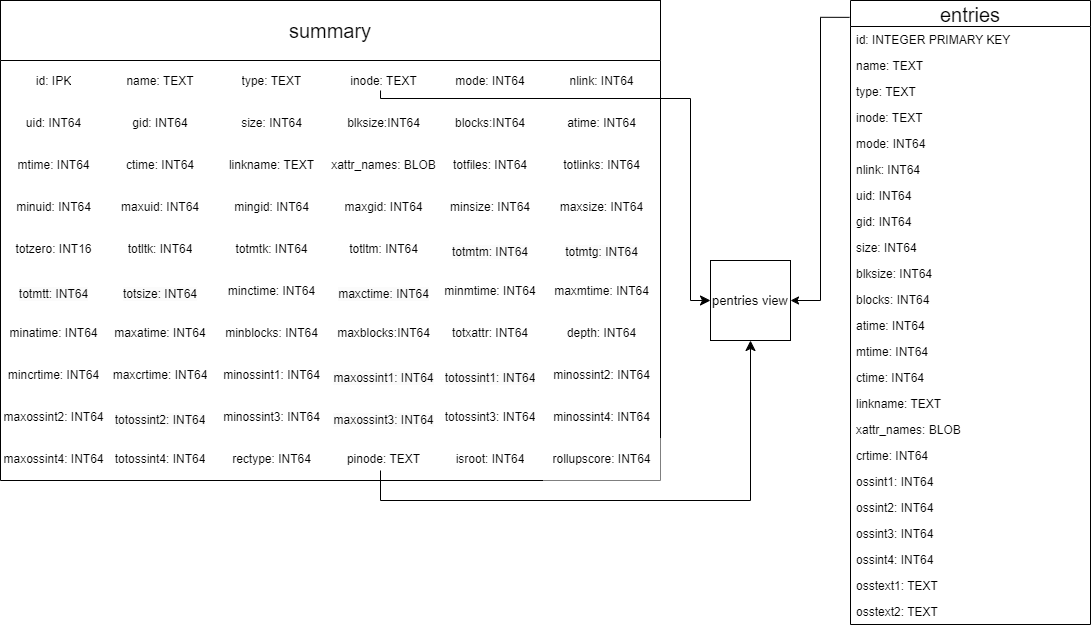
\includegraphics[width=1.0\textwidth]{images/Database_Schemas.png}
\caption{\label{fig:Database Schema}Database schema}
\end{figure}

\subsection{\pentries}
The original \pentries view was defined as:
\\\\
\texttt{SELECT entries.*, summary.inode AS pinode, summary.pinode AS
  ppinode FROM entries, summary};
\\\\
This was done in order to not store the parent inode of each entry,
which would be the same for every entry.

In general, users should query the \pentries view over the \entries
table in order to obtain complete sets of data to query on.

\subsubsection{\pentriesrollup}
In order to simplify rolling up indexes (see
Section~\ref{sec:rollup}), the \pentries view was modified to also
union with the \pentriesrollup table, which contains all child
\pentries views copied into the current directory's database file.

\subsection{\vrsummary}
The \vrsummary view is the \summary table with a handful of columns
repeated as aliases. This was done so that the \texttt{rpath} SQL
function can be called to generate the path of a given directory with
the same view and query whether or not the index has been rolled up,
and thus should be preferred over querying the \summary table. Using
the \summary table directly with a rolled up index is possible, but
will complicate queries.

\subsection{\vrpentries}
The \vrpentries view is the \pentries view with a few \summary table
columns aliased. This allows for the \texttt{rpath} SQL function can
be called to generate the path of a given directory with the same view
and query whether or not the index has been rolled up, and thus should
be preferred over querying \entries and \pentries. \texttt{rpath} with
the \vrpentries view is called with the same arguments that are used
with \vrsummary. Using the \pentries view directly with a rolled up
index is possible, but will complicate queries.

\subsection{\treesummary}
Similar to the directory \summary table, GUFI also provides
functionality to generate \treesummary tables. Instead of summarizing
only the data found in the entries table of the current directory, the
\treesummary table summarizes the contents of the entire subtree,
allowing for queries to completely skip processing entire
subtrees. See Section~\ref{sec:treesummary} for details.

\subsection{\vsummarydir}
The \vsummarydir view provides access to the entire directory summary
and not a partial directory summary (say by user or group).

\subsection{\vsummaryuser}
The \vsummaryuser view provides access to the directory summary for
each user (if this summary has been populated (not by default but
easily populatable via a query)).

\subsection{\vsummarygroup}
The \vsummarygroup view provides access to the directory summary for
each group (if this summary row has been created (not by default but
easily created via a query)).

\subsection{\vtsummarydir}
The vtsummarydir view provides access to the entire tree directory
summary and not a partial directory summary (say by user or group).

\subsection{\vtsummaryuser}
The \vtsummaryuser view provides access to the tree directory summary
for each user (if this summary row has been created (not by default
but easily created via a query)).

\subsection{\vtsummarygroup}
The \vtsummarygroup view provides access to the tree directory summary
for each group (if this summary has been populated (not by default but
easily populatable via a query)).

\subsection{\xattrs}
With the addition of extended attributes support, several more tables
and views were added into db.db. Additional database files with
different schemas were also added. See Section~\ref{sec:xattr_schema}
for details.

% This file is part of GUFI, which is part of MarFS, which is released
% under the BSD license.
%
%
% Copyright (c) 2017, Los Alamos National Security (LANS), LLC
% All rights reserved.
%
% Redistribution and use in source and binary forms, with or without modification,
% are permitted provided that the following conditions are met:
%
% 1. Redistributions of source code must retain the above copyright notice, this
% list of conditions and the following disclaimer.
%
% 2. Redistributions in binary form must reproduce the above copyright notice,
% this list of conditions and the following disclaimer in the documentation and/or
% other materials provided with the distribution.
%
% 3. Neither the name of the copyright holder nor the names of its contributors
% may be used to endorse or promote products derived from this software without
% specific prior written permission.
%
% THIS SOFTWARE IS PROVIDED BY THE COPYRIGHT HOLDERS AND CONTRIBUTORS "AS IS" AND
% ANY EXPRESS OR IMPLIED WARRANTIES, INCLUDING, BUT NOT LIMITED TO, THE IMPLIED
% WARRANTIES OF MERCHANTABILITY AND FITNESS FOR A PARTICULAR PURPOSE ARE DISCLAIMED.
% IN NO EVENT SHALL THE COPYRIGHT HOLDER OR CONTRIBUTORS BE LIABLE FOR ANY DIRECT,
% INDIRECT, INCIDENTAL, SPECIAL, EXEMPLARY, OR CONSEQUENTIAL DAMAGES (INCLUDING,
% BUT NOT LIMITED TO, PROCUREMENT OF SUBSTITUTE GOODS OR SERVICES; LOSS OF USE,
% DATA, OR PROFITS; OR BUSINESS INTERRUPTION) HOWEVER CAUSED AND ON ANY THEORY OF
% LIABILITY, WHETHER IN CONTRACT, STRICT LIABILITY, OR TORT (INCLUDING NEGLIGENCE
% OR OTHERWISE) ARISING IN ANY WAY OUT OF THE USE OF THIS SOFTWARE, EVEN IF
% ADVISED OF THE POSSIBILITY OF SUCH DAMAGE.
%
%
% From Los Alamos National Security, LLC:
% LA-CC-15-039
%
% Copyright (c) 2017, Los Alamos National Security, LLC All rights reserved.
% Copyright 2017. Los Alamos National Security, LLC. This software was produced
% under U.S. Government contract DE-AC52-06NA25396 for Los Alamos National
% Laboratory (LANL), which is operated by Los Alamos National Security, LLC for
% the U.S. Department of Energy. The U.S. Government has rights to use,
% reproduce, and distribute this software.  NEITHER THE GOVERNMENT NOR LOS
% ALAMOS NATIONAL SECURITY, LLC MAKES ANY WARRANTY, EXPRESS OR IMPLIED, OR
% ASSUMES ANY LIABILITY FOR THE USE OF THIS SOFTWARE.  If software is
% modified to produce derivative works, such modified software should be
% clearly marked, so as not to confuse it with the version available from
% LANL.
%
% THIS SOFTWARE IS PROVIDED BY LOS ALAMOS NATIONAL SECURITY, LLC AND CONTRIBUTORS
% "AS IS" AND ANY EXPRESS OR IMPLIED WARRANTIES, INCLUDING, BUT NOT LIMITED TO,
% THE IMPLIED WARRANTIES OF MERCHANTABILITY AND FITNESS FOR A PARTICULAR PURPOSE
% ARE DISCLAIMED. IN NO EVENT SHALL LOS ALAMOS NATIONAL SECURITY, LLC OR
% CONTRIBUTORS BE LIABLE FOR ANY DIRECT, INDIRECT, INCIDENTAL, SPECIAL,
% EXEMPLARY, OR CONSEQUENTIAL DAMAGES (INCLUDING, BUT NOT LIMITED TO, PROCUREMENT
% OF SUBSTITUTE GOODS OR SERVICES; LOSS OF USE, DATA, OR PROFITS; OR BUSINESS
% INTERRUPTION) HOWEVER CAUSED AND ON ANY THEORY OF LIABILITY, WHETHER IN
% CONTRACT, STRICT LIABILITY, OR TORT (INCLUDING NEGLIGENCE OR OTHERWISE) ARISING
% IN ANY WAY OUT OF THE USE OF THIS SOFTWARE, EVEN IF ADVISED OF THE POSSIBILITY
% OF SUCH DAMAGE.



\section{Indexing}
The first step to using GUFI is indexing a source filesystem.

An index created by GUFI retains the shape of the source filesystem:
directories that exist in the source filesystem also exist in the
index. If an administrator created the index, the directories will
also have the same access permissions, uid, and gid.

Indexes will not contain any of the files that the source filesystem
contained. Instead, all metadata extracted from a single directory of
the source filesystem will be placed into a single database file,
called db.db, in the cooresponding directory in the index. Each
database file will be created with a fixed schema that includes the
tables listed in Sections \ref{sec:schema} and
\ref{sec:xattr_schema}. Additional database files may be created if
extended attributes are extracted (see Section~\ref{sec:xattrs}).

Index processing (creation) occurs on a per-directory basis, and thus
is highly parallelizable.

\subsection{Directly Indexing a Filesystem}
% This file is part of GUFI, which is part of MarFS, which is released
% under the BSD license.
%
%
% Copyright (c) 2017, Los Alamos National Security (LANS), LLC
% All rights reserved.
%
% Redistribution and use in source and binary forms, with or without modification,
% are permitted provided that the following conditions are met:
%
% 1. Redistributions of source code must retain the above copyright notice, this
% list of conditions and the following disclaimer.
%
% 2. Redistributions in binary form must reproduce the above copyright notice,
% this list of conditions and the following disclaimer in the documentation and/or
% other materials provided with the distribution.
%
% 3. Neither the name of the copyright holder nor the names of its contributors
% may be used to endorse or promote products derived from this software without
% specific prior written permission.
%
% THIS SOFTWARE IS PROVIDED BY THE COPYRIGHT HOLDERS AND CONTRIBUTORS "AS IS" AND
% ANY EXPRESS OR IMPLIED WARRANTIES, INCLUDING, BUT NOT LIMITED TO, THE IMPLIED
% WARRANTIES OF MERCHANTABILITY AND FITNESS FOR A PARTICULAR PURPOSE ARE DISCLAIMED.
% IN NO EVENT SHALL THE COPYRIGHT HOLDER OR CONTRIBUTORS BE LIABLE FOR ANY DIRECT,
% INDIRECT, INCIDENTAL, SPECIAL, EXEMPLARY, OR CONSEQUENTIAL DAMAGES (INCLUDING,
% BUT NOT LIMITED TO, PROCUREMENT OF SUBSTITUTE GOODS OR SERVICES; LOSS OF USE,
% DATA, OR PROFITS; OR BUSINESS INTERRUPTION) HOWEVER CAUSED AND ON ANY THEORY OF
% LIABILITY, WHETHER IN CONTRACT, STRICT LIABILITY, OR TORT (INCLUDING NEGLIGENCE
% OR OTHERWISE) ARISING IN ANY WAY OUT OF THE USE OF THIS SOFTWARE, EVEN IF
% ADVISED OF THE POSSIBILITY OF SUCH DAMAGE.
%
%
% From Los Alamos National Security, LLC:
% LA-CC-15-039
%
% Copyright (c) 2017, Los Alamos National Security, LLC All rights reserved.
% Copyright 2017. Los Alamos National Security, LLC. This software was produced
% under U.S. Government contract DE-AC52-06NA25396 for Los Alamos National
% Laboratory (LANL), which is operated by Los Alamos National Security, LLC for
% the U.S. Department of Energy. The U.S. Government has rights to use,
% reproduce, and distribute this software.  NEITHER THE GOVERNMENT NOR LOS
% ALAMOS NATIONAL SECURITY, LLC MAKES ANY WARRANTY, EXPRESS OR IMPLIED, OR
% ASSUMES ANY LIABILITY FOR THE USE OF THIS SOFTWARE.  If software is
% modified to produce derivative works, such modified software should be
% clearly marked, so as not to confuse it with the version available from
% LANL.
%
% THIS SOFTWARE IS PROVIDED BY LOS ALAMOS NATIONAL SECURITY, LLC AND CONTRIBUTORS
% "AS IS" AND ANY EXPRESS OR IMPLIED WARRANTIES, INCLUDING, BUT NOT LIMITED TO,
% THE IMPLIED WARRANTIES OF MERCHANTABILITY AND FITNESS FOR A PARTICULAR PURPOSE
% ARE DISCLAIMED. IN NO EVENT SHALL LOS ALAMOS NATIONAL SECURITY, LLC OR
% CONTRIBUTORS BE LIABLE FOR ANY DIRECT, INDIRECT, INCIDENTAL, SPECIAL,
% EXEMPLARY, OR CONSEQUENTIAL DAMAGES (INCLUDING, BUT NOT LIMITED TO, PROCUREMENT
% OF SUBSTITUTE GOODS OR SERVICES; LOSS OF USE, DATA, OR PROFITS; OR BUSINESS
% INTERRUPTION) HOWEVER CAUSED AND ON ANY THEORY OF LIABILITY, WHETHER IN
% CONTRACT, STRICT LIABILITY, OR TORT (INCLUDING NEGLIGENCE OR OTHERWISE) ARISING
% IN ANY WAY OUT OF THE USE OF THIS SOFTWARE, EVEN IF ADVISED OF THE POSSIBILITY
% OF SUCH DAMAGE.



\subsubsection{\gufidirindex}
\gufidirindex is used to directly create an index based off of the
contents of a provided directory.

\begin{table} [h]
  \centering
  \begin{tabular}{l|l}
    Flag & Functionality \\
    \hline
    -h & help manual \\
    \hline
    -H & Show assigned input values \\
    \hline
    -n \textless num\_threads\textgreater & define number of threads to use \\
    \hline
    -x & pull xattrs from source file-sys into GUFI \\
    \hline
    -z \textless max\_level\textgreater & maximum level to go down to \\
    \hline
    -k \textless filename\textgreater & file containing directory names to skip \\
    \hline
    -M \textless bytes\textgreater & target memory footprint \\
    \hline
    -C \textless count\textgreater & Number of subdirectories allowed to be \\
                                   & enqueued for parallel processing. Any \\
                                   & remainders will be processed in-situ \\
    \hline
    -e & compress work items \\
    \hline
  \end{tabular}
  \caption{\label{fig:Flags_for_dir2index} \gufidirindex Flags and Arguments}
\end{table}

\begin{figure} [h]
  \centering
  \includegraphics[width=1.0\textwidth]{images/gufi_dir2index.png}
  \caption{\label{fig:gufi_dir2index} \gufidirindex workflow}
\end{figure}

\paragraph{Usage} ~\\\\
\gufidirindex \texttt{[flags] input\_dir... output\_dir} \\\\
The index of \texttt{input\_dir\textsubscript{i}} will be placed in \texttt{output\_dir/\$(basename input\_dir\textsubscript{i})}.

\subsection{Indirectly Indexing a Filesystem}
\input{sections/tracefile.tex}
% This file is part of GUFI, which is part of MarFS, which is released
% under the BSD license.
%
%
% Copyright (c) 2017, Los Alamos National Security (LANS), LLC
% All rights reserved.
%
% Redistribution and use in source and binary forms, with or without modification,
% are permitted provided that the following conditions are met:
%
% 1. Redistributions of source code must retain the above copyright notice, this
% list of conditions and the following disclaimer.
%
% 2. Redistributions in binary form must reproduce the above copyright notice,
% this list of conditions and the following disclaimer in the documentation and/or
% other materials provided with the distribution.
%
% 3. Neither the name of the copyright holder nor the names of its contributors
% may be used to endorse or promote products derived from this software without
% specific prior written permission.
%
% THIS SOFTWARE IS PROVIDED BY THE COPYRIGHT HOLDERS AND CONTRIBUTORS "AS IS" AND
% ANY EXPRESS OR IMPLIED WARRANTIES, INCLUDING, BUT NOT LIMITED TO, THE IMPLIED
% WARRANTIES OF MERCHANTABILITY AND FITNESS FOR A PARTICULAR PURPOSE ARE DISCLAIMED.
% IN NO EVENT SHALL THE COPYRIGHT HOLDER OR CONTRIBUTORS BE LIABLE FOR ANY DIRECT,
% INDIRECT, INCIDENTAL, SPECIAL, EXEMPLARY, OR CONSEQUENTIAL DAMAGES (INCLUDING,
% BUT NOT LIMITED TO, PROCUREMENT OF SUBSTITUTE GOODS OR SERVICES; LOSS OF USE,
% DATA, OR PROFITS; OR BUSINESS INTERRUPTION) HOWEVER CAUSED AND ON ANY THEORY OF
% LIABILITY, WHETHER IN CONTRACT, STRICT LIABILITY, OR TORT (INCLUDING NEGLIGENCE
% OR OTHERWISE) ARISING IN ANY WAY OUT OF THE USE OF THIS SOFTWARE, EVEN IF
% ADVISED OF THE POSSIBILITY OF SUCH DAMAGE.
%
%
% From Los Alamos National Security, LLC:
% LA-CC-15-039
%
% Copyright (c) 2017, Los Alamos National Security, LLC All rights reserved.
% Copyright 2017. Los Alamos National Security, LLC. This software was produced
% under U.S. Government contract DE-AC52-06NA25396 for Los Alamos National
% Laboratory (LANL), which is operated by Los Alamos National Security, LLC for
% the U.S. Department of Energy. The U.S. Government has rights to use,
% reproduce, and distribute this software.  NEITHER THE GOVERNMENT NOR LOS
% ALAMOS NATIONAL SECURITY, LLC MAKES ANY WARRANTY, EXPRESS OR IMPLIED, OR
% ASSUMES ANY LIABILITY FOR THE USE OF THIS SOFTWARE.  If software is
% modified to produce derivative works, such modified software should be
% clearly marked, so as not to confuse it with the version available from
% LANL.
%
% THIS SOFTWARE IS PROVIDED BY LOS ALAMOS NATIONAL SECURITY, LLC AND CONTRIBUTORS
% "AS IS" AND ANY EXPRESS OR IMPLIED WARRANTIES, INCLUDING, BUT NOT LIMITED TO,
% THE IMPLIED WARRANTIES OF MERCHANTABILITY AND FITNESS FOR A PARTICULAR PURPOSE
% ARE DISCLAIMED. IN NO EVENT SHALL LOS ALAMOS NATIONAL SECURITY, LLC OR
% CONTRIBUTORS BE LIABLE FOR ANY DIRECT, INDIRECT, INCIDENTAL, SPECIAL,
% EXEMPLARY, OR CONSEQUENTIAL DAMAGES (INCLUDING, BUT NOT LIMITED TO, PROCUREMENT
% OF SUBSTITUTE GOODS OR SERVICES; LOSS OF USE, DATA, OR PROFITS; OR BUSINESS
% INTERRUPTION) HOWEVER CAUSED AND ON ANY THEORY OF LIABILITY, WHETHER IN
% CONTRACT, STRICT LIABILITY, OR TORT (INCLUDING NEGLIGENCE OR OTHERWISE) ARISING
% IN ANY WAY OUT OF THE USE OF THIS SOFTWARE, EVEN IF ADVISED OF THE POSSIBILITY
% OF SUCH DAMAGE.



\subsubsection{\gufidirtrace}
\gufidirtrace generates trace files to allow for indexes to be easily
transfered to different locations rather than requiring entire trees
to be copied around.

\begin{table} [htb]
  \centering
  \begin{tabular}{l|l}
    Flag & Functionality \\
    \hline
    -h & help manual \\
    \hline
    -H & Show assigned input values \\
    \hline
    -n \textless num\_threads\textgreater & define number of threads to use \\
    \hline
    -x & pull xattrs from source file-sys into GUFI \\
    \hline
    -d \textless delim\textgreater & delimiter (one char)  [use 'x' for 0x1E] \\
    \hline
    -k \textless filename\textgreater & file containing directory names to skip \\
    \hline
    -M \textless bytes\textgreater & target memory footprint \\
    \hline
    -C \textless count\textgreater & Number of subdirectories allowed to be \\
                                   & enqueued for parallel processing. Any \\
                                   & remainders will be processed in-situ \\
    \hline
    -e & compress work items \\
    \hline
    -q \textless basename\textgreater & Mapping of basename of file to keep track of \\
    \ \ \ \ \textless attachname\textgreater & during indexing to attachname at query time \\
    \hline
  \end{tabular}
  \caption{\label{fig:Flags_for_dir2trace} \gufidirtrace Flags and Arguments}
\end{table}

\paragraph{Usage} ~\\\\
\gufidirtrace \texttt{[flags] input\_dir... output\_prefix} \\\\
Trace files with the name \texttt{output\_prefix.\$\{i\}}, where i $\in$ [0, number of threads), will be created.

% This file is part of GUFI, which is part of MarFS, which is released
% under the BSD license.
%
%
% Copyright (c) 2017, Los Alamos National Security (LANS), LLC
% All rights reserved.
%
% Redistribution and use in source and binary forms, with or without modification,
% are permitted provided that the following conditions are met:
%
% 1. Redistributions of source code must retain the above copyright notice, this
% list of conditions and the following disclaimer.
%
% 2. Redistributions in binary form must reproduce the above copyright notice,
% this list of conditions and the following disclaimer in the documentation and/or
% other materials provided with the distribution.
%
% 3. Neither the name of the copyright holder nor the names of its contributors
% may be used to endorse or promote products derived from this software without
% specific prior written permission.
%
% THIS SOFTWARE IS PROVIDED BY THE COPYRIGHT HOLDERS AND CONTRIBUTORS "AS IS" AND
% ANY EXPRESS OR IMPLIED WARRANTIES, INCLUDING, BUT NOT LIMITED TO, THE IMPLIED
% WARRANTIES OF MERCHANTABILITY AND FITNESS FOR A PARTICULAR PURPOSE ARE DISCLAIMED.
% IN NO EVENT SHALL THE COPYRIGHT HOLDER OR CONTRIBUTORS BE LIABLE FOR ANY DIRECT,
% INDIRECT, INCIDENTAL, SPECIAL, EXEMPLARY, OR CONSEQUENTIAL DAMAGES (INCLUDING,
% BUT NOT LIMITED TO, PROCUREMENT OF SUBSTITUTE GOODS OR SERVICES; LOSS OF USE,
% DATA, OR PROFITS; OR BUSINESS INTERRUPTION) HOWEVER CAUSED AND ON ANY THEORY OF
% LIABILITY, WHETHER IN CONTRACT, STRICT LIABILITY, OR TORT (INCLUDING NEGLIGENCE
% OR OTHERWISE) ARISING IN ANY WAY OUT OF THE USE OF THIS SOFTWARE, EVEN IF
% ADVISED OF THE POSSIBILITY OF SUCH DAMAGE.
%
%
% From Los Alamos National Security, LLC:
% LA-CC-15-039
%
% Copyright (c) 2017, Los Alamos National Security, LLC All rights reserved.
% Copyright 2017. Los Alamos National Security, LLC. This software was produced
% under U.S. Government contract DE-AC52-06NA25396 for Los Alamos National
% Laboratory (LANL), which is operated by Los Alamos National Security, LLC for
% the U.S. Department of Energy. The U.S. Government has rights to use,
% reproduce, and distribute this software.  NEITHER THE GOVERNMENT NOR LOS
% ALAMOS NATIONAL SECURITY, LLC MAKES ANY WARRANTY, EXPRESS OR IMPLIED, OR
% ASSUMES ANY LIABILITY FOR THE USE OF THIS SOFTWARE.  If software is
% modified to produce derivative works, such modified software should be
% clearly marked, so as not to confuse it with the version available from
% LANL.
%
% THIS SOFTWARE IS PROVIDED BY LOS ALAMOS NATIONAL SECURITY, LLC AND CONTRIBUTORS
% "AS IS" AND ANY EXPRESS OR IMPLIED WARRANTIES, INCLUDING, BUT NOT LIMITED TO,
% THE IMPLIED WARRANTIES OF MERCHANTABILITY AND FITNESS FOR A PARTICULAR PURPOSE
% ARE DISCLAIMED. IN NO EVENT SHALL LOS ALAMOS NATIONAL SECURITY, LLC OR
% CONTRIBUTORS BE LIABLE FOR ANY DIRECT, INDIRECT, INCIDENTAL, SPECIAL,
% EXEMPLARY, OR CONSEQUENTIAL DAMAGES (INCLUDING, BUT NOT LIMITED TO, PROCUREMENT
% OF SUBSTITUTE GOODS OR SERVICES; LOSS OF USE, DATA, OR PROFITS; OR BUSINESS
% INTERRUPTION) HOWEVER CAUSED AND ON ANY THEORY OF LIABILITY, WHETHER IN
% CONTRACT, STRICT LIABILITY, OR TORT (INCLUDING NEGLIGENCE OR OTHERWISE) ARISING
% IN ANY WAY OUT OF THE USE OF THIS SOFTWARE, EVEN IF ADVISED OF THE POSSIBILITY
% OF SUCH DAMAGE.



\subsubsection{\gufitraceindex}
\gufitraceindex is used to convert trace files into indexes. It is
essentially the same as \gufidirindex except it obtains data from
trace files instead of the filesystem being indexed.

Per thread trace files may be passed into \gufitraceindex
directly. Note that passing in too many trace files at once might
result in running out of file descriptors. Alternatively, the per
thread trace files may be concatenated in any order into a smaller
number of larger files for processing.

Extended attributes will be processed if they are found in the traces.
There is no need to tell \gufitraceindex to process them
with \texttt{-x}.

\begin{table} [htb]
  \centering
  \begin{tabular}{l|l}
    Flag & Functionality \\
    \hline
    -h & help manual \\
    \hline
    -H & Show assigned input values \\
    \hline
    -n \textless num\_threads\textgreater & define number of threads to use \\
    \hline
    -d \textless delim\textgreater & delimiter (one char)  [use 'x' for 0x1E] \\
    \hline
    -M \textless bytes\textgreater & target memory footprint \\
    \hline
  \end{tabular}
  \caption{\label{fig:Flags_for_dir2trace} \gufidirtrace Flags and Arguments}
\end{table}

\paragraph{Usage} ~\\\\
\gufitraceindex \texttt{[flags] trace\_file... index\_root} \\\\
Each source filesystem found in the trace files will be converted to an index placed underneath \texttt{output\_dir}.

% This file is part of GUFI, which is part of MarFS, which is released
% under the BSD license.
%
%
% Copyright (c) 2017, Los Alamos National Security (LANS), LLC
% All rights reserved.
%
% Redistribution and use in source and binary forms, with or without modification,
% are permitted provided that the following conditions are met:
%
% 1. Redistributions of source code must retain the above copyright notice, this
% list of conditions and the following disclaimer.
%
% 2. Redistributions in binary form must reproduce the above copyright notice,
% this list of conditions and the following disclaimer in the documentation and/or
% other materials provided with the distribution.
%
% 3. Neither the name of the copyright holder nor the names of its contributors
% may be used to endorse or promote products derived from this software without
% specific prior written permission.
%
% THIS SOFTWARE IS PROVIDED BY THE COPYRIGHT HOLDERS AND CONTRIBUTORS "AS IS" AND
% ANY EXPRESS OR IMPLIED WARRANTIES, INCLUDING, BUT NOT LIMITED TO, THE IMPLIED
% WARRANTIES OF MERCHANTABILITY AND FITNESS FOR A PARTICULAR PURPOSE ARE DISCLAIMED.
% IN NO EVENT SHALL THE COPYRIGHT HOLDER OR CONTRIBUTORS BE LIABLE FOR ANY DIRECT,
% INDIRECT, INCIDENTAL, SPECIAL, EXEMPLARY, OR CONSEQUENTIAL DAMAGES (INCLUDING,
% BUT NOT LIMITED TO, PROCUREMENT OF SUBSTITUTE GOODS OR SERVICES; LOSS OF USE,
% DATA, OR PROFITS; OR BUSINESS INTERRUPTION) HOWEVER CAUSED AND ON ANY THEORY OF
% LIABILITY, WHETHER IN CONTRACT, STRICT LIABILITY, OR TORT (INCLUDING NEGLIGENCE
% OR OTHERWISE) ARISING IN ANY WAY OUT OF THE USE OF THIS SOFTWARE, EVEN IF
% ADVISED OF THE POSSIBILITY OF SUCH DAMAGE.
%
%
% From Los Alamos National Security, LLC:
% LA-CC-15-039
%
% Copyright (c) 2017, Los Alamos National Security, LLC All rights reserved.
% Copyright 2017. Los Alamos National Security, LLC. This software was produced
% under U.S. Government contract DE-AC52-06NA25396 for Los Alamos National
% Laboratory (LANL), which is operated by Los Alamos National Security, LLC for
% the U.S. Department of Energy. The U.S. Government has rights to use,
% reproduce, and distribute this software.  NEITHER THE GOVERNMENT NOR LOS
% ALAMOS NATIONAL SECURITY, LLC MAKES ANY WARRANTY, EXPRESS OR IMPLIED, OR
% ASSUMES ANY LIABILITY FOR THE USE OF THIS SOFTWARE.  If software is
% modified to produce derivative works, such modified software should be
% clearly marked, so as not to confuse it with the version available from
% LANL.
%
% THIS SOFTWARE IS PROVIDED BY LOS ALAMOS NATIONAL SECURITY, LLC AND CONTRIBUTORS
% "AS IS" AND ANY EXPRESS OR IMPLIED WARRANTIES, INCLUDING, BUT NOT LIMITED TO,
% THE IMPLIED WARRANTIES OF MERCHANTABILITY AND FITNESS FOR A PARTICULAR PURPOSE
% ARE DISCLAIMED. IN NO EVENT SHALL LOS ALAMOS NATIONAL SECURITY, LLC OR
% CONTRIBUTORS BE LIABLE FOR ANY DIRECT, INDIRECT, INCIDENTAL, SPECIAL,
% EXEMPLARY, OR CONSEQUENTIAL DAMAGES (INCLUDING, BUT NOT LIMITED TO, PROCUREMENT
% OF SUBSTITUTE GOODS OR SERVICES; LOSS OF USE, DATA, OR PROFITS; OR BUSINESS
% INTERRUPTION) HOWEVER CAUSED AND ON ANY THEORY OF LIABILITY, WHETHER IN
% CONTRACT, STRICT LIABILITY, OR TORT (INCLUDING NEGLIGENCE OR OTHERWISE) ARISING
% IN ANY WAY OUT OF THE USE OF THIS SOFTWARE, EVEN IF ADVISED OF THE POSSIBILITY
% OF SUCH DAMAGE.



\subsection{Extended Attributes}
\label{sec:xattrs}
GUFI supports the indexing and querying of extended attributes
(xattrs).

Reading standard filesystem permissions of files only requires read
(and execute) access to the directory. Extended attribute names are
visible this way. However, because xattr values are user defined data,
their permissions are checked at the file level, requiring changes to
how GUFI stores data. For more information on xattrs, see
\texttt{xattr(7)}, \listxattr, and \getxattr.

Directories containing files from multiple users might have xattrs
that are not readable by all who can view the \lstat data of the
directory. As GUFI was originally designed to only use directory-level
permission checks, a number of modifications were made to process
xattrs without violating their permissions.

\subsubsection{Roll In}
Extended attributes that are readable by all who have access to the
directory are stored in the \xattrspwd table in the main
database. These xattrs are referred to as ``rolled in''.

The rules that determine whether or not an xattr pair can roll in are
as follows:

\begin{itemize}
\item File is 0+R
\item File is UG+R doesnt matter on other, with file and parent same
  usr and grp and parent has only UG+R with no other read
\item File is U+R doesnt matter on grp and other, with file and parent
  same usr and parent dir has only U+R, no grp and other read
\item Directory has write for every read:
    \texttt{drw*rw*rw*} or \texttt{drw*rw*\_\_\_} or
    \texttt{drw*\_\_\_\_\_\_} - if you can write the dir you can
    chmod the files to see the xattrs
\end{itemize}

Extended attributes that cannot be read by all who can read the
directory are stored in external per-uid and per-gid databases set
with \texttt{uid:nobody} and \texttt{nobody:gid} owners
respectively. This makes it so that non-admin users cannot access the
xattrs stored in external databases that they do not have permissions
to access.

\subsubsection{Schema}
\label{sec:xattr_schema}
The main database and all external databases contain the following
tables and views with the 3 columns \texttt{inode}, \texttt{name}, and
\texttt{value}:

\begin{itemize}
\item The \xattrspwd table contains all extended attributes of the
  current directory that were placed into this database file.

\item The \xattrsrollup table contains all extended attributes that
  were placed into the children directories that were subsequently
  rolled up into the current directory.

\item The \xattrsavail view is the union of all extended attributes
  in \xattrspwd and \xattrsrollup in this database file.
\end{itemize}

Additionally, each main database file has the following tables and
views in order to keep track of which files were created by GUFI for
the purposes of storing xattrs:

\begin{itemize}
\item The \xattrfilespwd table contains a listing of external database
  filenames that contain xattrs that were not rolled in.
\item The \xattrfilesrollup table contains a listing of external
  database filenames that contain xattrs that were not
  rolled in, but were brought in by rolling up.
\item The \xattrfiles view combines the listings of database filenames
  found in \xattrfilespwd and \xattrfilesrollup.
\end{itemize}

\subsubsection{Usage}
Extended attributes are not pulled from the filesystem by default. In
order to pull them, pass \texttt{-x} to \gufidirindex or
\gufidirtrace.

Note that only xattr pairs in the user namespace (\texttt{user.*}) are
extracted.


\subsection{Location}
GUFI is expected to be used to query the indexes of many filesystems
all at once. However, the source filesystems are not expected to be
accessible from each other. In order for the indexes from many
disconnected systems to be queried at once, they should all be built
under a common directory on a single machine.

\subsubsection{Permissions}
If a GUFI tree is located on a different machine than the source
tree, the users and groups are probably not available on the machine
with the index on it. \texttt{/etc/passwd} should be populated with
the entries from the source machine and modified so that they do not
have a home directory, and are not allowed to log in
(\texttt{/sbin/nologin}). Similarly, \texttt{/etc/group} should be
updated with the source machine's groups and modified to remove any
unnecessary information.

% This file is part of GUFI, which is part of MarFS, which is released
% under the BSD license.
%
%
% Copyright (c) 2017, Los Alamos National Security (LANS), LLC
% All rights reserved.
%
% Redistribution and use in source and binary forms, with or without modification,
% are permitted provided that the following conditions are met:
%
% 1. Redistributions of source code must retain the above copyright notice, this
% list of conditions and the following disclaimer.
%
% 2. Redistributions in binary form must reproduce the above copyright notice,
% this list of conditions and the following disclaimer in the documentation and/or
% other materials provided with the distribution.
%
% 3. Neither the name of the copyright holder nor the names of its contributors
% may be used to endorse or promote products derived from this software without
% specific prior written permission.
%
% THIS SOFTWARE IS PROVIDED BY THE COPYRIGHT HOLDERS AND CONTRIBUTORS "AS IS" AND
% ANY EXPRESS OR IMPLIED WARRANTIES, INCLUDING, BUT NOT LIMITED TO, THE IMPLIED
% WARRANTIES OF MERCHANTABILITY AND FITNESS FOR A PARTICULAR PURPOSE ARE DISCLAIMED.
% IN NO EVENT SHALL THE COPYRIGHT HOLDER OR CONTRIBUTORS BE LIABLE FOR ANY DIRECT,
% INDIRECT, INCIDENTAL, SPECIAL, EXEMPLARY, OR CONSEQUENTIAL DAMAGES (INCLUDING,
% BUT NOT LIMITED TO, PROCUREMENT OF SUBSTITUTE GOODS OR SERVICES; LOSS OF USE,
% DATA, OR PROFITS; OR BUSINESS INTERRUPTION) HOWEVER CAUSED AND ON ANY THEORY OF
% LIABILITY, WHETHER IN CONTRACT, STRICT LIABILITY, OR TORT (INCLUDING NEGLIGENCE
% OR OTHERWISE) ARISING IN ANY WAY OUT OF THE USE OF THIS SOFTWARE, EVEN IF
% ADVISED OF THE POSSIBILITY OF SUCH DAMAGE.
%
%
% From Los Alamos National Security, LLC:
% LA-CC-15-039
%
% Copyright (c) 2017, Los Alamos National Security, LLC All rights reserved.
% Copyright 2017. Los Alamos National Security, LLC. This software was produced
% under U.S. Government contract DE-AC52-06NA25396 for Los Alamos National
% Laboratory (LANL), which is operated by Los Alamos National Security, LLC for
% the U.S. Department of Energy. The U.S. Government has rights to use,
% reproduce, and distribute this software.  NEITHER THE GOVERNMENT NOR LOS
% ALAMOS NATIONAL SECURITY, LLC MAKES ANY WARRANTY, EXPRESS OR IMPLIED, OR
% ASSUMES ANY LIABILITY FOR THE USE OF THIS SOFTWARE.  If software is
% modified to produce derivative works, such modified software should be
% clearly marked, so as not to confuse it with the version available from
% LANL.
%
% THIS SOFTWARE IS PROVIDED BY LOS ALAMOS NATIONAL SECURITY, LLC AND CONTRIBUTORS
% "AS IS" AND ANY EXPRESS OR IMPLIED WARRANTIES, INCLUDING, BUT NOT LIMITED TO,
% THE IMPLIED WARRANTIES OF MERCHANTABILITY AND FITNESS FOR A PARTICULAR PURPOSE
% ARE DISCLAIMED. IN NO EVENT SHALL LOS ALAMOS NATIONAL SECURITY, LLC OR
% CONTRIBUTORS BE LIABLE FOR ANY DIRECT, INDIRECT, INCIDENTAL, SPECIAL,
% EXEMPLARY, OR CONSEQUENTIAL DAMAGES (INCLUDING, BUT NOT LIMITED TO, PROCUREMENT
% OF SUBSTITUTE GOODS OR SERVICES; LOSS OF USE, DATA, OR PROFITS; OR BUSINESS
% INTERRUPTION) HOWEVER CAUSED AND ON ANY THEORY OF LIABILITY, WHETHER IN
% CONTRACT, STRICT LIABILITY, OR TORT (INCLUDING NEGLIGENCE OR OTHERWISE) ARISING
% IN ANY WAY OUT OF THE USE OF THIS SOFTWARE, EVEN IF ADVISED OF THE POSSIBILITY
% OF SUCH DAMAGE.



\section{Post-Indexing}
After indexing, additional operations can be performed on the index in
order to increase query performance.

% This file is part of GUFI, which is part of MarFS, which is released
% under the BSD license.
%
%
% Copyright (c) 2017, Los Alamos National Security (LANS), LLC
% All rights reserved.
%
% Redistribution and use in source and binary forms, with or without modification,
% are permitted provided that the following conditions are met:
%
% 1. Redistributions of source code must retain the above copyright notice, this
% list of conditions and the following disclaimer.
%
% 2. Redistributions in binary form must reproduce the above copyright notice,
% this list of conditions and the following disclaimer in the documentation and/or
% other materials provided with the distribution.
%
% 3. Neither the name of the copyright holder nor the names of its contributors
% may be used to endorse or promote products derived from this software without
% specific prior written permission.
%
% THIS SOFTWARE IS PROVIDED BY THE COPYRIGHT HOLDERS AND CONTRIBUTORS "AS IS" AND
% ANY EXPRESS OR IMPLIED WARRANTIES, INCLUDING, BUT NOT LIMITED TO, THE IMPLIED
% WARRANTIES OF MERCHANTABILITY AND FITNESS FOR A PARTICULAR PURPOSE ARE DISCLAIMED.
% IN NO EVENT SHALL THE COPYRIGHT HOLDER OR CONTRIBUTORS BE LIABLE FOR ANY DIRECT,
% INDIRECT, INCIDENTAL, SPECIAL, EXEMPLARY, OR CONSEQUENTIAL DAMAGES (INCLUDING,
% BUT NOT LIMITED TO, PROCUREMENT OF SUBSTITUTE GOODS OR SERVICES; LOSS OF USE,
% DATA, OR PROFITS; OR BUSINESS INTERRUPTION) HOWEVER CAUSED AND ON ANY THEORY OF
% LIABILITY, WHETHER IN CONTRACT, STRICT LIABILITY, OR TORT (INCLUDING NEGLIGENCE
% OR OTHERWISE) ARISING IN ANY WAY OUT OF THE USE OF THIS SOFTWARE, EVEN IF
% ADVISED OF THE POSSIBILITY OF SUCH DAMAGE.
%
%
% From Los Alamos National Security, LLC:
% LA-CC-15-039
%
% Copyright (c) 2017, Los Alamos National Security, LLC All rights reserved.
% Copyright 2017. Los Alamos National Security, LLC. This software was produced
% under U.S. Government contract DE-AC52-06NA25396 for Los Alamos National
% Laboratory (LANL), which is operated by Los Alamos National Security, LLC for
% the U.S. Department of Energy. The U.S. Government has rights to use,
% reproduce, and distribute this software.  NEITHER THE GOVERNMENT NOR LOS
% ALAMOS NATIONAL SECURITY, LLC MAKES ANY WARRANTY, EXPRESS OR IMPLIED, OR
% ASSUMES ANY LIABILITY FOR THE USE OF THIS SOFTWARE.  If software is
% modified to produce derivative works, such modified software should be
% clearly marked, so as not to confuse it with the version available from
% LANL.
%
% THIS SOFTWARE IS PROVIDED BY LOS ALAMOS NATIONAL SECURITY, LLC AND CONTRIBUTORS
% "AS IS" AND ANY EXPRESS OR IMPLIED WARRANTIES, INCLUDING, BUT NOT LIMITED TO,
% THE IMPLIED WARRANTIES OF MERCHANTABILITY AND FITNESS FOR A PARTICULAR PURPOSE
% ARE DISCLAIMED. IN NO EVENT SHALL LOS ALAMOS NATIONAL SECURITY, LLC OR
% CONTRIBUTORS BE LIABLE FOR ANY DIRECT, INDIRECT, INCIDENTAL, SPECIAL,
% EXEMPLARY, OR CONSEQUENTIAL DAMAGES (INCLUDING, BUT NOT LIMITED TO, PROCUREMENT
% OF SUBSTITUTE GOODS OR SERVICES; LOSS OF USE, DATA, OR PROFITS; OR BUSINESS
% INTERRUPTION) HOWEVER CAUSED AND ON ANY THEORY OF LIABILITY, WHETHER IN
% CONTRACT, STRICT LIABILITY, OR TORT (INCLUDING NEGLIGENCE OR OTHERWISE) ARISING
% IN ANY WAY OUT OF THE USE OF THIS SOFTWARE, EVEN IF ADVISED OF THE POSSIBILITY
% OF SUCH DAMAGE.



\subsection{Rollup}
\label{sec:rollup}
Rolling up is a major optimization that can reduce the number of
directories that need to be opened when querying by significant
amounts while still obtaining the same results as an unmodified index.

\subsubsection{Bottlenecks}
During querying, every single directory runs a fixed set of
operations:

\begin{itemize}
  \item \texttt{opendir(3)}
  \item \texttt{readdir(3)} (Looped)
  \item \texttt{sqlite3\_open\_v2}
  \item \texttt{sqlite3\_exec\_v2}
  \item \texttt{sqlite3\_close(3)}
  \item \texttt{closedir(3)}
\end{itemize}

Each of these operations have costs associated with them. Some are
fixed and some depend on the shape and contents of the index. Reducing
the number of directories processed allows for fixed costs to be
amortized.

\subsubsection{Rules}
\label{sec:rolluprules}
\paragraph{Whether or not a directory {\it CAN} roll up} ~\\
In order for a child directory to be allowed to roll up into its
parent directory, it must follow two rules. First, all of its children
must be rolled up. Second, all of its children must have permissions
that satisfy any one of the following conditions with the parent.

\begin{itemize}
  \item World readable and executable (o+rx)
  \item Matching user, group, and others permissions, with the same
    user and group
  \item Matching user and group permissions, readable and executable
    (ug+rx) with the same user and group, and not world readable and
    excutable (o-rx)
  \item Matching user permissions, readable and executable (u+rx) with
    the same user and not group or world readable and executable
    (go-rx)
\end{itemize}

Note that because leaf directories have no children with which to have
conflicting permission with, they are considered rolled up.

\paragraph{Whether or not a directory {\it SHOULD} roll up} ~\\
In addition to the permission-based rules that determine whether or
not a directory can roll up, we also have a small check to say whether
or not a directory should roll up.

As data is rolled upwards in the index, databases towards the top will
accumulate more and more data from its subtrees. If directories are
allowed to roll up without limit, some databases will become
significantly larger than others, causing large amounts of tail
latency.

The \gufirollup executable has the \texttt{-L} flag that limits the number
of entries that may be found within a single directory.

\subsubsection{Steps}
The processing of rolling up involves a number of steps that update
the tables of the parent directory.

First, the target directory is checked to ensure it can and should
roll up its children into itself using the rules listed in
\ref{sec:rolluprules}. If rollup will proceed, the parent's \summary table
is updated with a rollup score of 1.

Then, the contents each child is copied into the parent:

\begin{enumerate}
\item The child's \pentries view is copied into the parent's
  \pentriesrollup table. The parent's \pentries view is updated
  automatically.
\item The child's \summary table is copied into the parent's \summary
  table with the names of each child directory prefixed with the parent's
  name.
\end{enumerate}

Rolling up can be viewed as flattening the contents of the index while
taking into consideration the permissions of each directory.

Rolling up will cause the size of the index to grow significantly due
to the amount of data being replicated. One obvious optimization would
be to only roll up to the top-most level where a directory can roll up
to (one extra copy of the subtree instead of repeated copies). This
however, will only allow for queries to take advantage of rollups if
they start above the top-most rollup directory. Starting a query below
the top-most rollup level would result in the original subtree's query
time whereas the implemented method of rolling up allows for queries
starting at any point in the index to take advantage of rollups.

The rollup operation can take some time, and so indicies are not
rolled up automatically. The \gufirollup executable must be called
manually.

\subsubsection{Extended Attributes}
Additional steps are needed to rollup xattrs:

\begin{itemize}
\item The child's \xattrsavail view (without external database data)
  is copied into the parent's \xattrsrollup table.
\item The child's \xattrfiles view (without external databases data)
  is copied into the parent's \xattrfilesrollup table.
\item The child's external database files are copied into the
  parent. If the parent already has an external database file with the
  same uid or gid, the contents of the external database are copied
  into the parent's external database's \xattrsrollup table instead.
\end{itemize}

\subsubsection{Schema Usage}
Prior to rolling up, the \pentries view can be treated as an optional
improvement to the \entries table. After rolling up, the \pentries
view will have been updated extensively and will contain both the
original \entries data as well as the rolled up data. However, the
\vrpentries view should be preferred over the \pentries view. The
\vrpentries view contains data from the \summary table that allows for
the parent directory of each entry's row to be generated when the
index is rolled up, rather than requiring users to do it themselves,
which is error prone. The \vrpentries view can be used whether or not
the index has been rolled up, and should be the preferred view for
getting file and link data.

Similarly, the \vrsummary view should be preferred over the \summary
table whether or not the index has been rolled up, as it works in both
cases.

The \vrpentries and \vrsummary views were constructed specifically to
make the usage of the \rpath SQL function consistent. See the
\rpath entry in Table~\ref{tab:sqlwcontext} for details.

\subsubsection{\gufirollup executable}
In order to apply rollup to an index, run the \gufirollup executable:
\\\\
\indent \gufirollup \texttt{index\_root}
\\\\
Figure~\ref{fig:rollupworkflow} shows the overall structure of the
\gufirollup executable. \gufirollup recursively descends the index and
performs the rollup operation on a directory once all of the
directory's children have been processed as shown in
Figure~\ref{fig:rollupfunction}.

\begin{sidewaysfigure} [hp]
  \centering \includegraphics[width=\textwidth]{images/rollup.png}
  \caption{\gufirollup Workflow}
  \label{fig:rollupworkflow}
\end{sidewaysfigure}

\begin{figure} [hp]
  \centering
  \includegraphics[width=\textwidth]{images/rollup_function.png}
  \caption{Rollup Function Diagram}
  \label{fig:rollupfunction}
\end{figure}

\subsubsection{Undoing a rollup}
To remove rollup data from an index, run the \gufiunrollup executable:
\\\\
\indent \gufiunrollup \texttt{index\_root}

% This file is part of GUFI, which is part of MarFS, which is released
% under the BSD license.
%
%
% Copyright (c) 2017, Los Alamos National Security (LANS), LLC
% All rights reserved.
%
% Redistribution and use in source and binary forms, with or without modification,
% are permitted provided that the following conditions are met:
%
% 1. Redistributions of source code must retain the above copyright notice, this
% list of conditions and the following disclaimer.
%
% 2. Redistributions in binary form must reproduce the above copyright notice,
% this list of conditions and the following disclaimer in the documentation and/or
% other materials provided with the distribution.
%
% 3. Neither the name of the copyright holder nor the names of its contributors
% may be used to endorse or promote products derived from this software without
% specific prior written permission.
%
% THIS SOFTWARE IS PROVIDED BY THE COPYRIGHT HOLDERS AND CONTRIBUTORS "AS IS" AND
% ANY EXPRESS OR IMPLIED WARRANTIES, INCLUDING, BUT NOT LIMITED TO, THE IMPLIED
% WARRANTIES OF MERCHANTABILITY AND FITNESS FOR A PARTICULAR PURPOSE ARE DISCLAIMED.
% IN NO EVENT SHALL THE COPYRIGHT HOLDER OR CONTRIBUTORS BE LIABLE FOR ANY DIRECT,
% INDIRECT, INCIDENTAL, SPECIAL, EXEMPLARY, OR CONSEQUENTIAL DAMAGES (INCLUDING,
% BUT NOT LIMITED TO, PROCUREMENT OF SUBSTITUTE GOODS OR SERVICES; LOSS OF USE,
% DATA, OR PROFITS; OR BUSINESS INTERRUPTION) HOWEVER CAUSED AND ON ANY THEORY OF
% LIABILITY, WHETHER IN CONTRACT, STRICT LIABILITY, OR TORT (INCLUDING NEGLIGENCE
% OR OTHERWISE) ARISING IN ANY WAY OUT OF THE USE OF THIS SOFTWARE, EVEN IF
% ADVISED OF THE POSSIBILITY OF SUCH DAMAGE.
%
%
% From Los Alamos National Security, LLC:
% LA-CC-15-039
%
% Copyright (c) 2017, Los Alamos National Security, LLC All rights reserved.
% Copyright 2017. Los Alamos National Security, LLC. This software was produced
% under U.S. Government contract DE-AC52-06NA25396 for Los Alamos National
% Laboratory (LANL), which is operated by Los Alamos National Security, LLC for
% the U.S. Department of Energy. The U.S. Government has rights to use,
% reproduce, and distribute this software.  NEITHER THE GOVERNMENT NOR LOS
% ALAMOS NATIONAL SECURITY, LLC MAKES ANY WARRANTY, EXPRESS OR IMPLIED, OR
% ASSUMES ANY LIABILITY FOR THE USE OF THIS SOFTWARE.  If software is
% modified to produce derivative works, such modified software should be
% clearly marked, so as not to confuse it with the version available from
% LANL.
%
% THIS SOFTWARE IS PROVIDED BY LOS ALAMOS NATIONAL SECURITY, LLC AND CONTRIBUTORS
% "AS IS" AND ANY EXPRESS OR IMPLIED WARRANTIES, INCLUDING, BUT NOT LIMITED TO,
% THE IMPLIED WARRANTIES OF MERCHANTABILITY AND FITNESS FOR A PARTICULAR PURPOSE
% ARE DISCLAIMED. IN NO EVENT SHALL LOS ALAMOS NATIONAL SECURITY, LLC OR
% CONTRIBUTORS BE LIABLE FOR ANY DIRECT, INDIRECT, INCIDENTAL, SPECIAL,
% EXEMPLARY, OR CONSEQUENTIAL DAMAGES (INCLUDING, BUT NOT LIMITED TO, PROCUREMENT
% OF SUBSTITUTE GOODS OR SERVICES; LOSS OF USE, DATA, OR PROFITS; OR BUSINESS
% INTERRUPTION) HOWEVER CAUSED AND ON ANY THEORY OF LIABILITY, WHETHER IN
% CONTRACT, STRICT LIABILITY, OR TORT (INCLUDING NEGLIGENCE OR OTHERWISE) ARISING
% IN ANY WAY OUT OF THE USE OF THIS SOFTWARE, EVEN IF ADVISED OF THE POSSIBILITY
% OF SUCH DAMAGE.



\subsection{Generate \treesummary Tables}
\label{sec:treesummary}
The \treesummary table is an optional table that is placed into
db.db. It contains a summary of the entire subtree starting at current
directory using minimums, maximums, and totals of numerical values.

When a query is provided to \gufiquery \texttt{-T}, the \treesummary
table is queried first. Because \treesummary tables do not necessarily
exist, \gufiquery first checks for the existence of the \treesummary
table in the directory being processed before performing the
\texttt{-T} query. If the \texttt{-T} query returns no results, the
entire subtree will be skipped.

\subsubsection{\gufitreesummary}
Starting from a directory provided in the command line,
\gufitreesummary recursively traverses to the bottom of the tree,
collecting data from the \summary table of each child directory
database. If a \treesummary table is discovered in a subdirectory,
descent down the tree is stopped as the \treesummary table contains
all of the information about that directory as well as all
subdirectories underneath it. Once all of the data has been collected,
it is summarized and placed into the \treesummary table of the
starting directory.

Generating \treesummary tables for all directories using this top-down
approach will take a long time due to the repeated traversals across
the same directories. Because of this, \gufitreesummary generates the
\treesummary table for the provided directory only.

If generating \treesummary tables using \gufitreesummary, the tables
should be generated at optimal points within the index. For example,
if the index is on a home directory, it may be useful to generate
\treesummary tables at each user's home directory.
\\\\
Example Call:
\\\\
\indent \gufitreesummary \texttt{index\_root}

\subsubsection{\gufitreesummaryall}
\gufitreesummaryall generates \treesummary tables for all
directories. This is done by walking to the bottom of the tree and
generating \treesummary tables while walking back up, which only
occurs after all subdirectories have had their \treesummary tables
generated. Leaf directories, by definition, do not have
subdirectories, and further traversal down is unnecessary and
impossible. Their \treesummary tables are thus duplicates of their
\summary tables, providing the base case for the walk back up the
tree. Directories above the leaves can then use the \treesummary data
found in their immediate subdirectories, which are 1) guaranteed to
exist and 2) guaranteed to summarize the entire subdirectory's
subtree, to generate their own \treesummary tables.
\\\\
Example Call:
\\\\
\indent \gufitreesummaryall \texttt{index\_root}

\subsubsection{\gufirollup}
Just as with \gufitreesummaryall, rolling up a tree involves walking
to the bottom of the tree and working upwards. This allows for
\treesummary generation to be performed automatically during the roll
up operation, resulting in \treesummary tables being generated for all
directories whether or not they were rolled up.


% This file is part of GUFI, which is part of MarFS, which is released
% under the BSD license.
%
%
% Copyright (c) 2017, Los Alamos National Security (LANS), LLC
% All rights reserved.
%
% Redistribution and use in source and binary forms, with or without modification,
% are permitted provided that the following conditions are met:
%
% 1. Redistributions of source code must retain the above copyright notice, this
% list of conditions and the following disclaimer.
%
% 2. Redistributions in binary form must reproduce the above copyright notice,
% this list of conditions and the following disclaimer in the documentation and/or
% other materials provided with the distribution.
%
% 3. Neither the name of the copyright holder nor the names of its contributors
% may be used to endorse or promote products derived from this software without
% specific prior written permission.
%
% THIS SOFTWARE IS PROVIDED BY THE COPYRIGHT HOLDERS AND CONTRIBUTORS "AS IS" AND
% ANY EXPRESS OR IMPLIED WARRANTIES, INCLUDING, BUT NOT LIMITED TO, THE IMPLIED
% WARRANTIES OF MERCHANTABILITY AND FITNESS FOR A PARTICULAR PURPOSE ARE DISCLAIMED.
% IN NO EVENT SHALL THE COPYRIGHT HOLDER OR CONTRIBUTORS BE LIABLE FOR ANY DIRECT,
% INDIRECT, INCIDENTAL, SPECIAL, EXEMPLARY, OR CONSEQUENTIAL DAMAGES (INCLUDING,
% BUT NOT LIMITED TO, PROCUREMENT OF SUBSTITUTE GOODS OR SERVICES; LOSS OF USE,
% DATA, OR PROFITS; OR BUSINESS INTERRUPTION) HOWEVER CAUSED AND ON ANY THEORY OF
% LIABILITY, WHETHER IN CONTRACT, STRICT LIABILITY, OR TORT (INCLUDING NEGLIGENCE
% OR OTHERWISE) ARISING IN ANY WAY OUT OF THE USE OF THIS SOFTWARE, EVEN IF
% ADVISED OF THE POSSIBILITY OF SUCH DAMAGE.
%
%
% From Los Alamos National Security, LLC:
% LA-CC-15-039
%
% Copyright (c) 2017, Los Alamos National Security, LLC All rights reserved.
% Copyright 2017. Los Alamos National Security, LLC. This software was produced
% under U.S. Government contract DE-AC52-06NA25396 for Los Alamos National
% Laboratory (LANL), which is operated by Los Alamos National Security, LLC for
% the U.S. Department of Energy. The U.S. Government has rights to use,
% reproduce, and distribute this software.  NEITHER THE GOVERNMENT NOR LOS
% ALAMOS NATIONAL SECURITY, LLC MAKES ANY WARRANTY, EXPRESS OR IMPLIED, OR
% ASSUMES ANY LIABILITY FOR THE USE OF THIS SOFTWARE.  If software is
% modified to produce derivative works, such modified software should be
% clearly marked, so as not to confuse it with the version available from
% LANL.
%
% THIS SOFTWARE IS PROVIDED BY LOS ALAMOS NATIONAL SECURITY, LLC AND CONTRIBUTORS
% "AS IS" AND ANY EXPRESS OR IMPLIED WARRANTIES, INCLUDING, BUT NOT LIMITED TO,
% THE IMPLIED WARRANTIES OF MERCHANTABILITY AND FITNESS FOR A PARTICULAR PURPOSE
% ARE DISCLAIMED. IN NO EVENT SHALL LOS ALAMOS NATIONAL SECURITY, LLC OR
% CONTRIBUTORS BE LIABLE FOR ANY DIRECT, INDIRECT, INCIDENTAL, SPECIAL,
% EXEMPLARY, OR CONSEQUENTIAL DAMAGES (INCLUDING, BUT NOT LIMITED TO, PROCUREMENT
% OF SUBSTITUTE GOODS OR SERVICES; LOSS OF USE, DATA, OR PROFITS; OR BUSINESS
% INTERRUPTION) HOWEVER CAUSED AND ON ANY THEORY OF LIABILITY, WHETHER IN
% CONTRACT, STRICT LIABILITY, OR TORT (INCLUDING NEGLIGENCE OR OTHERWISE) ARISING
% IN ANY WAY OUT OF THE USE OF THIS SOFTWARE, EVEN IF ADVISED OF THE POSSIBILITY
% OF SUCH DAMAGE.



\section{Querying}
Once a GUFI tree with one or more indexes has been created, it should
be queried using GUFI tools and SQL statements.

% This file is part of GUFI, which is part of MarFS, which is released
% under the BSD license.
%
%
% Copyright (c) 2017, Los Alamos National Security (LANS), LLC
% All rights reserved.
%
% Redistribution and use in source and binary forms, with or without modification,
% are permitted provided that the following conditions are met:
%
% 1. Redistributions of source code must retain the above copyright notice, this
% list of conditions and the following disclaimer.
%
% 2. Redistributions in binary form must reproduce the above copyright notice,
% this list of conditions and the following disclaimer in the documentation and/or
% other materials provided with the distribution.
%
% 3. Neither the name of the copyright holder nor the names of its contributors
% may be used to endorse or promote products derived from this software without
% specific prior written permission.
%
% THIS SOFTWARE IS PROVIDED BY THE COPYRIGHT HOLDERS AND CONTRIBUTORS "AS IS" AND
% ANY EXPRESS OR IMPLIED WARRANTIES, INCLUDING, BUT NOT LIMITED TO, THE IMPLIED
% WARRANTIES OF MERCHANTABILITY AND FITNESS FOR A PARTICULAR PURPOSE ARE DISCLAIMED.
% IN NO EVENT SHALL THE COPYRIGHT HOLDER OR CONTRIBUTORS BE LIABLE FOR ANY DIRECT,
% INDIRECT, INCIDENTAL, SPECIAL, EXEMPLARY, OR CONSEQUENTIAL DAMAGES (INCLUDING,
% BUT NOT LIMITED TO, PROCUREMENT OF SUBSTITUTE GOODS OR SERVICES; LOSS OF USE,
% DATA, OR PROFITS; OR BUSINESS INTERRUPTION) HOWEVER CAUSED AND ON ANY THEORY OF
% LIABILITY, WHETHER IN CONTRACT, STRICT LIABILITY, OR TORT (INCLUDING NEGLIGENCE
% OR OTHERWISE) ARISING IN ANY WAY OUT OF THE USE OF THIS SOFTWARE, EVEN IF
% ADVISED OF THE POSSIBILITY OF SUCH DAMAGE.
%
%
% From Los Alamos National Security, LLC:
% LA-CC-15-039
%
% Copyright (c) 2017, Los Alamos National Security, LLC All rights reserved.
% Copyright 2017. Los Alamos National Security, LLC. This software was produced
% under U.S. Government contract DE-AC52-06NA25396 for Los Alamos National
% Laboratory (LANL), which is operated by Los Alamos National Security, LLC for
% the U.S. Department of Energy. The U.S. Government has rights to use,
% reproduce, and distribute this software.  NEITHER THE GOVERNMENT NOR LOS
% ALAMOS NATIONAL SECURITY, LLC MAKES ANY WARRANTY, EXPRESS OR IMPLIED, OR
% ASSUMES ANY LIABILITY FOR THE USE OF THIS SOFTWARE.  If software is
% modified to produce derivative works, such modified software should be
% clearly marked, so as not to confuse it with the version available from
% LANL.
%
% THIS SOFTWARE IS PROVIDED BY LOS ALAMOS NATIONAL SECURITY, LLC AND CONTRIBUTORS
% "AS IS" AND ANY EXPRESS OR IMPLIED WARRANTIES, INCLUDING, BUT NOT LIMITED TO,
% THE IMPLIED WARRANTIES OF MERCHANTABILITY AND FITNESS FOR A PARTICULAR PURPOSE
% ARE DISCLAIMED. IN NO EVENT SHALL LOS ALAMOS NATIONAL SECURITY, LLC OR
% CONTRIBUTORS BE LIABLE FOR ANY DIRECT, INDIRECT, INCIDENTAL, SPECIAL,
% EXEMPLARY, OR CONSEQUENTIAL DAMAGES (INCLUDING, BUT NOT LIMITED TO, PROCUREMENT
% OF SUBSTITUTE GOODS OR SERVICES; LOSS OF USE, DATA, OR PROFITS; OR BUSINESS
% INTERRUPTION) HOWEVER CAUSED AND ON ANY THEORY OF LIABILITY, WHETHER IN
% CONTRACT, STRICT LIABILITY, OR TORT (INCLUDING NEGLIGENCE OR OTHERWISE) ARISING
% IN ANY WAY OUT OF THE USE OF THIS SOFTWARE, EVEN IF ADVISED OF THE POSSIBILITY
% OF SUCH DAMAGE.



\subsection{\gufiquery}

\gufiquery is the main tool used for accessing indexes.

\gufiquery processes each directory in parallel, passing user provided
SQL statements to the current directory's database. Because of this,
callers will need to know about GUFI's database and table schemas. We
expect only ``advanced'' users such as administrators and developers
to use \gufiquery directly. Users who do not know how GUFI functions
may call \gufiquery, but might not be able to use it properly.

\subsubsection{Flags}

\begin{table}[H]
  \centering
  \begin{tabular*}{\linewidth}{l|p{0.5\linewidth}}
    Flag & Functionality \\
    \hline
    -h & help \\
    \hline
    -H & show assigned input values (debugging) \\
    \hline
    -E \textless SQL ent\textgreater & SQL for entries table \\
    \hline
    -S \textless SQL sum\textgreater & SQL for summary table \\
    \hline
    -T \textless SQL tsum\textgreater & SQL for tree-summary table \\
    \hline
    -a & AND/OR (SQL query combination) \\
    \hline
    -n \textless threads\textgreater & number of threads (default: 1) \\
    \hline
    -j & print the information in terse form \\
    \hline
    -o \textless out\_fname\textgreater & output file (one-per thread, with thread-id suffix) \\
    \hline
    -d \textless delim\textgreater & one char delimiter (default: \texttt{\textbackslash x1E}) \\
    \hline
    -O \textless out\_DB\textgreater & output DB \\
    \hline
    -I \textless SQL\_init\textgreater & SQL init \\
    \hline
    -F \textless SQL\_fin\textgreater & SQL cleanup \\
    \hline
    -y \textless min-level\textgreater & minimum level to descend to \\
    \hline
    -z \textless max-level\textgreater & maximum level to descend to \\
    \hline
    -J \textless SQL\_interm\textgreater & SQL for intermediate
    results (no default. ex.: \texttt{INSERT INTO \textless
      aggregate table name\textgreater \ SELECT * FROM \textless
      intermediate table name\textgreater}) \\
    \hline
    -K \textless create aggregate\textgreater & SQL to create the final aggregation table \\
    \hline
    -G \textless SQL\_aggregate\textgreater & SQL for aggregated
    results (no default. ex.: \texttt{SELECT * FROM
      \textless aggregate table name\textgreater}) \\
    \hline
    -m & Keep mtime and atime same on the database files \\
    \hline
    -B \textless buffer size\textgreater & size of each thread's output buffer in bytes \\
    \hline
    -w & open the database files in read-write mode instead of read only mode \\
    \hline
    -x & enable xattr processing \\
    \hline
    -k & file containing directory names to skip \\
    \hline
    -M \textless bytes\textgreater & target memory footprint \\
    \hline
    -e & compress work items \\
    \hline
  \end{tabular*}
  \caption{\label{tab:widgets} \gufiquery Flags and Arguments}
\end{table}

\subsubsection{Flag/Table Associations}
A \gufiquery call should use at least one of the \texttt{-T},
\texttt{-S}, and \texttt{-E} flags to pass in SQL
statements\footnote{Not passing in any SQL statements results in
  \gufiquery simply walking the tree and filling up the inode and
  dentries caches.}.

\begin{itemize}
\item \texttt{-T} should be used to query the \treesummary table.
\item \texttt{-S} should be used to query the \summary table and its
  variants.
\item \texttt{-E} should be used to query the \entries table and its
  variants.
\end{itemize}

Note that user provided SQL statements are passed directly into
SQLite\footnote{Anything that can be done with SQL can also be done on
  the databases in an index. To prevent accidental modifications,
  databases default to opening in read-only mode.} and thus
associations between flags and tables are not
enforced\footnote{Querying tables/views with the wrong flags may
  result in unexpected output.}.

Prior to rolling up, the \pentries view can be treated as an optional
improvement to the \entries table. After rolling up, the \pentries
view will have been updated extensively and will contain both the
original \entries data as well as the rolled up data. Querying the
\entries table of a rolled up index will return a subset of the total
results that exist in the index since it only contains the current
directory's information and subdirectories are not traversed. The
\summary table was updated directly, so querying it will return all
directory information.

However, instead of querying the \summary table and switching between
querying \entries and \pentries, the \vrpentries and \vrsummary views
should always be used. These views contain data from the \summary
table that allow for the path of each row relative to the starting
path to be generated using the \rpath SQL function, whether or not the
index has been rolled up, with consistent input arguments (see
Table~\ref{tab:sqlwcontext} for details). These views and function
were set up to help simpliy the queries that users provide.

\subsubsection{Short Circuiting with Compound Queries}
At each directory, the set of user provided SQL statements run on the
db.db file in the following order: if \texttt{-T} was provided, it
will run if the optional \treesummary table exists in the database. If
\texttt{-T} was not run or returned at least one row of results,
\texttt{-S} will run if it was provided. If \texttt{-S} was not
provided or returned at least one row of results, \texttt{-E} will run
if it was provided.

Conversely, if \texttt{-T} runs and does not return any results,
processing is stopped before running the \texttt{-S} query. If
\texttt{-S} does not return any results, the \texttt{-E} query is not
run. This allows for threads to short circuit the processing of a
directory if it is determined early on that no rows would be obtained
from a later query. For example, if a query is searching for files
larger than 1MB, but the \texttt{-S} query found that the range of
file sizes is 1KB to 5KB, there is no need to run the \texttt{-E}
query to get rows, since no rows will match in any case.

To turn off short circuiting and always run all queries for each
directory, pass the \texttt{-a} flag to \gufiquery.

\subsubsection{Extended Attributes}
When querying for xattrs, pass \texttt{-x} to \gufiquery to build the
\xattrs view for querying. This view is a SQL union of rolled in
xattrs and any external databases that successfully
attaches. Attaching the database files checks the permissions of the
xattrs. \texttt{UNION} removes duplicate entries that showed up in
multiple external databases, leaving a unique set of xattrs accessible
by the caller.

The \xentries, \xpentries, \xsummary, \vrxpentries, and \vrxsummary
views are convenience views generated so that users do not have to
perform joins themselves. They are \entries, \pentries, \summary,
\vrpentries, and \vrsummary enhanced with the \texttt{xattr\_name} and
\texttt{xattr\_value} columns. Like the \xattrs view, these views are
also dropped at the end of directory processing.

Note that entries with multiple extended attributes will return
multiple times in this view.

\subsubsection{External Databases}
Attaching external data to GUFI allows for arbitrary data to be
associated with filesystem data. In order to remain flexible and not
prescribe schema requirements, using this feature is more complex than
using other GUFI features.

Each external database file is presented as a view concatentating it
to a table in the template database file. When a directory does not
have a database file specified for attaching to a given view, the view
is comprised of only the table from the template file.

Pass \texttt{-I} and \texttt{-Q} to \gufiquery. \texttt{-Q} has 4
positional arguments:

\begin{table}[h!]
  \centering
  \begin{tabular}{|l|l|}
    \hline
    \texttt{-Q} Argument & Explanation \\
    \hline
    \texttt{basename} & The basename of the database file in the current directory \\
                      & to attach \\
    \hline
    \texttt{table} & The table in the database file to attach \\
    \hline
    \texttt{template.table} & The template file's attach name (specified in \texttt{-I}) and table \\
                            & name with a matching schema \\
    \hline
    \texttt{view} & The name of the view that will be made available for \\
                  & \texttt{-T}, \texttt{-S}, and \texttt{-E} \\
    \hline
  \end{tabular}
\end{table}

Finally, in \texttt{-T}, \texttt{-S}, and \texttt{-E}, the caller
should join the view created in \texttt{-Q} with GUFI data to pull
what they are looking for. The recommended columns to join on are
\texttt{name} and \texttt{type} to reduce the likelihood of joining
to the wrong rows.
\\\\
Example Usage:
\begin{table}[H]
  \centering
  \begin{tabular}{ll}
    \gufiquery & \texttt{-I "ATTACH template.db AS template;"} \\
               & \texttt{-Q "external.db" "table" "template.table" "ext"} \\
               & \texttt{-E "SELECT * FROM pentries} \\
               & \texttt{\ \ \ \ LEFT JOIN ext ON (pentries.name == ext.name)} \\
               & \texttt{\ \ \ \ AND (pentries.type == ext.type);"} \\
               & \texttt{index\_root} \\
  \end{tabular}
\end{table}

For each \texttt{view} that is to be made available for querying,
\texttt{-I} should be updated with more \texttt{ATTACH} SQL
statements, another \texttt{-Q} should be passed in, and each query
flag should be updated to use the new views.
\\\\
Multiple External Databases Example:
\begin{table}[H]
  \centering
  \begin{tabular}{ll}
    \gufiquery & \texttt{-I "ATTACH template1.db AS template1;} \\
               & \texttt{\ \ \ \ ATTACH template2.db AS template2;"} \\
               & \texttt{-Q "externall.db" "table" "template1.table" "ext1"} \\
               & \texttt{-Q "external2.db" "table" "template2.table" "ext2"} \\
               & \texttt{-E "SELECT * FROM pentries} \\
               & \texttt{\ \ \ \ LEFT JOIN ext1 ON (pentries.name == ext1.name)} \\
               & \texttt{\ \ \ \ AND (pentries.type == ext1.type)} \\
               & \texttt{\ \ \ \ LEFT JOIN ext2 ON (pentries.name == ext2.name)} \\
               & \texttt{\ \ \ \ AND (pentries.type == ext2.type);"} \\
               & \texttt{index\_root} \\
  \end{tabular}
\end{table}

\subsubsection{Aggregation}
There are cases where independent per-thread results are not
desirable, such as when sorting or summing, where the results from
querying the index must be aggregated for final processing.

In order to handle these situations, the \texttt{-I} flag should be
used to create per-thread intermediate tables that are written to by
\texttt{-T}, \texttt{-S}, and \texttt{-E}. The intermediate table
results will then be aggregated using \texttt{-J} into the final table
created by \texttt{-K}. The rows stored in the final table are
processed one last time as a whole, rather than as results from
independent threads, using \texttt{-G}.

\subsubsection{Per-Thread Output Files}
The \texttt{-o} flag causes results to be outputted to text
files. When outputting in parallel, per-thread output files are
created with the thread id appended to the filename provided with the
flag. When aggregating, the aggregate results are written to the
filename specified by \texttt{-o} with no filename modifications.

\subsubsection{Per-Thread Output Database Files}
The \texttt{-O} flag allows for results to be written to SQLite
database files instead of text files. The resulting filenames follow
the same creation rules as \texttt{-o}. However, the queries passed
into \gufiquery need modifications. When writing in parallel,
\texttt{-I} is needed to create the table for each per-thread output
database. \texttt{-T}, \texttt{-S}, and \texttt{-E} should be modified
to write to the per-thread tables in the same way as writing to the
intermediate tables when aggregating. When writing aggregate results
to a database, \texttt{-G} is not needed as \texttt{-J} already wrote
the results into the aggregate table. However, \texttt{-G} may still
be provided to get results during the \gufiquery in addition to
queries on the results database file later on.

Output database files may be passed to the \querydbs executable for
further processing.

\subsubsection{Example Calls}

\begin{table}[H]
  \centering
  \caption{Parallel Results}
  \begin{tabular}{|l|l|}
    \hline
    Output     & \gufiquery \texttt{/path/to/index} \\
    \hline
    \stdout    & \texttt{-S "SELECT * FROM \vrsummary;"} \\
    \hline
    Per-thread & \texttt{-E "SELECT * FROM \vrpentries;"} \\
    Files      & \texttt{-o results} \\
    \hline
    Per-thread & \texttt{-I "CREATE  TABLE results(name TEXT, size INT64);"} \\
    Database   & \texttt{-S "INSERT INTO results SELECT name, size FROM \vrsummary;"} \\
    Files      & \texttt{-E "INSERT INTO results SELECT name, size FROM \vrpentries;"} \\
               & \texttt{-O results} \\
    \hline
  \end{tabular}
\end{table}

\begin{table}[H]
  \centering
  \caption{Aggregate Results}
  \begin{tabular}{|l|l|}
    \hline
    Output   & \gufiquery \texttt{/path/to/index} \\
    \hline
    \stdout  & \texttt{-I "CREATE TABLE intermediate(name TEXT, size INT64);"} \\
             & \texttt{-S "INSERT INTO intermediate SELECT name, size FROM \vrsummary;"} \\
             & \texttt{-K "CREATE TABLE aggregate(name TEXT, size INT64);"} \\
             & \texttt{-J "INSERT INSERT aggregate SELECT * FROM intermediate;"} \\
             & \texttt{-G "SELECT * FROM aggregate ORDER BY size DESC;"} \\
    \hline
    Single   & \texttt{-I "CREATE TABLE intermediate(name TEXT, size INT64);"} \\
    File     & \texttt{-E "INSERT INTO intermediate SELECT name, size FROM \vrpentries;"} \\
             & \texttt{-K "CREATE TABLE aggregate(name TEXT, size INT64);"} \\
             & \texttt{-J "INSERT INSERT aggregate SELECT * FROM intermediate;"} \\
             & \texttt{-G "SELECT * FROM aggregate ORDER BY size DESC;"} \\
             & \texttt{-o results} \\
    \hline
    Single   & \texttt{-I "CREATE TABLE intermediate(name TEXT, size INT64);"} \\
    Database & \texttt{-S "INSERT INTO intermediate SELECT name, size FROM \vrsummary;"} \\
    File     & \texttt{-E "INSERT INTO intermediate SELECT name, size FROM \vrpentries;"} \\
             & \texttt{-K "CREATE TABLE aggregate(name TEXT, size INT64);"} \\
             & \texttt{-J "INSERT INSERT aggregate SELECT * FROM intermediate;"} \\
             & \texttt{-O results} \\
    \hline
  \end{tabular}
\end{table}

\subsubsection{Behavior When Traversing Rolled Up Indexes}
When \gufiquery detects that a directory being processed has been
rolled up, the thread processing that directory does not enqueue work
to descend further down into the tree, as all of the data underneath
the current directory is available in the current directory. While
this may seem to only reduce tree traversal by ``some" amount, in
practise, rolling up indexes of real filesystems reduces the number of
directories (and thus the bottlenecks listed in
Section~\ref{subsec:bottlenecks}) that need to be processed by over
99\%, significantly reducing index query time.

Queries are not expected to have to change too often when switching
between unmodified indexes and rolled up indexes. If they do, they
should not have to change by much.

\subsubsection{Visualizing the Workflow}
\begin{figure}[H]
  \centering
  \includegraphics[width=\textwidth]{images/gufi_query_main.png}
  \caption{Workflow of \gufiquery}
\end{figure}

\paragraph{\processdir}
The core of \gufiquery is the \processdir function. This is where the
-T, -S, and -E flags are processed. Multiple instances of this
function are run in parallel via the thread pool in order to quickly
traverse and process an index.

\begin{figure}[H]
  \centering
  \includegraphics[width=\textwidth]{images/gufi_query_processdir.png}
  \caption{Workflow of \processdir}
\end{figure}

\paragraph{\querydb}
The \querydb macro is used to execute SQL statements and handle errors.

\begin{figure}[H]
  \centering
  \includegraphics[width=\textwidth]{images/querydb_macro.png}
  \caption{\querydb macro workflow}
\end{figure}

% This file is part of GUFI, which is part of MarFS, which is released
% under the BSD license.
%
%
% Copyright (c) 2017, Los Alamos National Security (LANS), LLC
% All rights reserved.
%
% Redistribution and use in source and binary forms, with or without modification,
% are permitted provided that the following conditions are met:
%
% 1. Redistributions of source code must retain the above copyright notice, this
% list of conditions and the following disclaimer.
%
% 2. Redistributions in binary form must reproduce the above copyright notice,
% this list of conditions and the following disclaimer in the documentation and/or
% other materials provided with the distribution.
%
% 3. Neither the name of the copyright holder nor the names of its contributors
% may be used to endorse or promote products derived from this software without
% specific prior written permission.
%
% THIS SOFTWARE IS PROVIDED BY THE COPYRIGHT HOLDERS AND CONTRIBUTORS "AS IS" AND
% ANY EXPRESS OR IMPLIED WARRANTIES, INCLUDING, BUT NOT LIMITED TO, THE IMPLIED
% WARRANTIES OF MERCHANTABILITY AND FITNESS FOR A PARTICULAR PURPOSE ARE DISCLAIMED.
% IN NO EVENT SHALL THE COPYRIGHT HOLDER OR CONTRIBUTORS BE LIABLE FOR ANY DIRECT,
% INDIRECT, INCIDENTAL, SPECIAL, EXEMPLARY, OR CONSEQUENTIAL DAMAGES (INCLUDING,
% BUT NOT LIMITED TO, PROCUREMENT OF SUBSTITUTE GOODS OR SERVICES; LOSS OF USE,
% DATA, OR PROFITS; OR BUSINESS INTERRUPTION) HOWEVER CAUSED AND ON ANY THEORY OF
% LIABILITY, WHETHER IN CONTRACT, STRICT LIABILITY, OR TORT (INCLUDING NEGLIGENCE
% OR OTHERWISE) ARISING IN ANY WAY OUT OF THE USE OF THIS SOFTWARE, EVEN IF
% ADVISED OF THE POSSIBILITY OF SUCH DAMAGE.
%
%
% From Los Alamos National Security, LLC:
% LA-CC-15-039
%
% Copyright (c) 2017, Los Alamos National Security, LLC All rights reserved.
% Copyright 2017. Los Alamos National Security, LLC. This software was produced
% under U.S. Government contract DE-AC52-06NA25396 for Los Alamos National
% Laboratory (LANL), which is operated by Los Alamos National Security, LLC for
% the U.S. Department of Energy. The U.S. Government has rights to use,
% reproduce, and distribute this software.  NEITHER THE GOVERNMENT NOR LOS
% ALAMOS NATIONAL SECURITY, LLC MAKES ANY WARRANTY, EXPRESS OR IMPLIED, OR
% ASSUMES ANY LIABILITY FOR THE USE OF THIS SOFTWARE.  If software is
% modified to produce derivative works, such modified software should be
% clearly marked, so as not to confuse it with the version available from
% LANL.
%
% THIS SOFTWARE IS PROVIDED BY LOS ALAMOS NATIONAL SECURITY, LLC AND CONTRIBUTORS
% "AS IS" AND ANY EXPRESS OR IMPLIED WARRANTIES, INCLUDING, BUT NOT LIMITED TO,
% THE IMPLIED WARRANTIES OF MERCHANTABILITY AND FITNESS FOR A PARTICULAR PURPOSE
% ARE DISCLAIMED. IN NO EVENT SHALL LOS ALAMOS NATIONAL SECURITY, LLC OR
% CONTRIBUTORS BE LIABLE FOR ANY DIRECT, INDIRECT, INCIDENTAL, SPECIAL,
% EXEMPLARY, OR CONSEQUENTIAL DAMAGES (INCLUDING, BUT NOT LIMITED TO, PROCUREMENT
% OF SUBSTITUTE GOODS OR SERVICES; LOSS OF USE, DATA, OR PROFITS; OR BUSINESS
% INTERRUPTION) HOWEVER CAUSED AND ON ANY THEORY OF LIABILITY, WHETHER IN
% CONTRACT, STRICT LIABILITY, OR TORT (INCLUDING NEGLIGENCE OR OTHERWISE) ARISING
% IN ANY WAY OUT OF THE USE OF THIS SOFTWARE, EVEN IF ADVISED OF THE POSSIBILITY
% OF SUCH DAMAGE.



\subsection{\querydbs}
\querydbs attaches all database files it is given into a single view
for querying. All tables in the provided database files should have
the same name and schema. For tables called \texttt{table}, the view
combining all tables will be named \texttt{vtable}. This was intended
to allow for easy post-processing of \gufiquery~\texttt{-O} output
database files.

\querydbs does not have a \texttt{gufi\_} prefix because it will work
for any set of input databases with the same schema. For example,
\querydbs can also be used directly on individual database files
from an index.

Note that there is a hard limit of 125 databases that can be queried
by querydbs that is set by SQLite3. This has been patched to 254,
making it less likely that directories run out of attaches.

% This file is part of GUFI, which is part of MarFS, which is released
% under the BSD license.
%
%
% Copyright (c) 2017, Los Alamos National Security (LANS), LLC
% All rights reserved.
%
% Redistribution and use in source and binary forms, with or without modification,
% are permitted provided that the following conditions are met:
%
% 1. Redistributions of source code must retain the above copyright notice, this
% list of conditions and the following disclaimer.
%
% 2. Redistributions in binary form must reproduce the above copyright notice,
% this list of conditions and the following disclaimer in the documentation and/or
% other materials provided with the distribution.
%
% 3. Neither the name of the copyright holder nor the names of its contributors
% may be used to endorse or promote products derived from this software without
% specific prior written permission.
%
% THIS SOFTWARE IS PROVIDED BY THE COPYRIGHT HOLDERS AND CONTRIBUTORS "AS IS" AND
% ANY EXPRESS OR IMPLIED WARRANTIES, INCLUDING, BUT NOT LIMITED TO, THE IMPLIED
% WARRANTIES OF MERCHANTABILITY AND FITNESS FOR A PARTICULAR PURPOSE ARE DISCLAIMED.
% IN NO EVENT SHALL THE COPYRIGHT HOLDER OR CONTRIBUTORS BE LIABLE FOR ANY DIRECT,
% INDIRECT, INCIDENTAL, SPECIAL, EXEMPLARY, OR CONSEQUENTIAL DAMAGES (INCLUDING,
% BUT NOT LIMITED TO, PROCUREMENT OF SUBSTITUTE GOODS OR SERVICES; LOSS OF USE,
% DATA, OR PROFITS; OR BUSINESS INTERRUPTION) HOWEVER CAUSED AND ON ANY THEORY OF
% LIABILITY, WHETHER IN CONTRACT, STRICT LIABILITY, OR TORT (INCLUDING NEGLIGENCE
% OR OTHERWISE) ARISING IN ANY WAY OUT OF THE USE OF THIS SOFTWARE, EVEN IF
% ADVISED OF THE POSSIBILITY OF SUCH DAMAGE.
%
%
% From Los Alamos National Security, LLC:
% LA-CC-15-039
%
% Copyright (c) 2017, Los Alamos National Security, LLC All rights reserved.
% Copyright 2017. Los Alamos National Security, LLC. This software was produced
% under U.S. Government contract DE-AC52-06NA25396 for Los Alamos National
% Laboratory (LANL), which is operated by Los Alamos National Security, LLC for
% the U.S. Department of Energy. The U.S. Government has rights to use,
% reproduce, and distribute this software.  NEITHER THE GOVERNMENT NOR LOS
% ALAMOS NATIONAL SECURITY, LLC MAKES ANY WARRANTY, EXPRESS OR IMPLIED, OR
% ASSUMES ANY LIABILITY FOR THE USE OF THIS SOFTWARE.  If software is
% modified to produce derivative works, such modified software should be
% clearly marked, so as not to confuse it with the version available from
% LANL.
%
% THIS SOFTWARE IS PROVIDED BY LOS ALAMOS NATIONAL SECURITY, LLC AND CONTRIBUTORS
% "AS IS" AND ANY EXPRESS OR IMPLIED WARRANTIES, INCLUDING, BUT NOT LIMITED TO,
% THE IMPLIED WARRANTIES OF MERCHANTABILITY AND FITNESS FOR A PARTICULAR PURPOSE
% ARE DISCLAIMED. IN NO EVENT SHALL LOS ALAMOS NATIONAL SECURITY, LLC OR
% CONTRIBUTORS BE LIABLE FOR ANY DIRECT, INDIRECT, INCIDENTAL, SPECIAL,
% EXEMPLARY, OR CONSEQUENTIAL DAMAGES (INCLUDING, BUT NOT LIMITED TO, PROCUREMENT
% OF SUBSTITUTE GOODS OR SERVICES; LOSS OF USE, DATA, OR PROFITS; OR BUSINESS
% INTERRUPTION) HOWEVER CAUSED AND ON ANY THEORY OF LIABILITY, WHETHER IN
% CONTRACT, STRICT LIABILITY, OR TORT (INCLUDING NEGLIGENCE OR OTHERWISE) ARISING
% IN ANY WAY OUT OF THE USE OF THIS SOFTWARE, EVEN IF ADVISED OF THE POSSIBILITY
% OF SUCH DAMAGE.



\subsection{\gufisqlite}
\gufisqlite is a simple program that imitates most of the
\texttt{sqlite3} cli while providing GUFI specific functions.  The
main difference from the \texttt{sqlite3} cli is that ''dot commands''
are not supported.

The difference between \gufisqlite and \querydbs is that \querydbs is
intended for parsing \gufiquery \texttt{-O} output, and has built-in
operations for automatically doing so, whereas \gufisqlite simply
forwards commands to \texttt{sqlite3}.

\subsubsection{Flags}
\begin{table} [H]
  \centering
  \begin{tabular}{l|l}
    Flag & Functionality \\
    \hline
    -h & help manual \\
    \hline
    -d \textless delim\textgreater & delimiter (one char)  [use 'x' for 0x1E] \\
    \hline
  \end{tabular}
  \caption{\gufisqlite Flags and Arguments}
\end{table}

\subsubsection{Usage}
\gufisqlite \texttt{[options] [db [SQL]...]}

If no SQL statements are passed in, SQL statements will be read in from stdin

% This file is part of GUFI, which is part of MarFS, which is released
% under the BSD license.
%
%
% Copyright (c) 2017, Los Alamos National Security (LANS), LLC
% All rights reserved.
%
% Redistribution and use in source and binary forms, with or without modification,
% are permitted provided that the following conditions are met:
%
% 1. Redistributions of source code must retain the above copyright notice, this
% list of conditions and the following disclaimer.
%
% 2. Redistributions in binary form must reproduce the above copyright notice,
% this list of conditions and the following disclaimer in the documentation and/or
% other materials provided with the distribution.
%
% 3. Neither the name of the copyright holder nor the names of its contributors
% may be used to endorse or promote products derived from this software without
% specific prior written permission.
%
% THIS SOFTWARE IS PROVIDED BY THE COPYRIGHT HOLDERS AND CONTRIBUTORS "AS IS" AND
% ANY EXPRESS OR IMPLIED WARRANTIES, INCLUDING, BUT NOT LIMITED TO, THE IMPLIED
% WARRANTIES OF MERCHANTABILITY AND FITNESS FOR A PARTICULAR PURPOSE ARE DISCLAIMED.
% IN NO EVENT SHALL THE COPYRIGHT HOLDER OR CONTRIBUTORS BE LIABLE FOR ANY DIRECT,
% INDIRECT, INCIDENTAL, SPECIAL, EXEMPLARY, OR CONSEQUENTIAL DAMAGES (INCLUDING,
% BUT NOT LIMITED TO, PROCUREMENT OF SUBSTITUTE GOODS OR SERVICES; LOSS OF USE,
% DATA, OR PROFITS; OR BUSINESS INTERRUPTION) HOWEVER CAUSED AND ON ANY THEORY OF
% LIABILITY, WHETHER IN CONTRACT, STRICT LIABILITY, OR TORT (INCLUDING NEGLIGENCE
% OR OTHERWISE) ARISING IN ANY WAY OUT OF THE USE OF THIS SOFTWARE, EVEN IF
% ADVISED OF THE POSSIBILITY OF SUCH DAMAGE.
%
%
% From Los Alamos National Security, LLC:
% LA-CC-15-039
%
% Copyright (c) 2017, Los Alamos National Security, LLC All rights reserved.
% Copyright 2017. Los Alamos National Security, LLC. This software was produced
% under U.S. Government contract DE-AC52-06NA25396 for Los Alamos National
% Laboratory (LANL), which is operated by Los Alamos National Security, LLC for
% the U.S. Department of Energy. The U.S. Government has rights to use,
% reproduce, and distribute this software.  NEITHER THE GOVERNMENT NOR LOS
% ALAMOS NATIONAL SECURITY, LLC MAKES ANY WARRANTY, EXPRESS OR IMPLIED, OR
% ASSUMES ANY LIABILITY FOR THE USE OF THIS SOFTWARE.  If software is
% modified to produce derivative works, such modified software should be
% clearly marked, so as not to confuse it with the version available from
% LANL.
%
% THIS SOFTWARE IS PROVIDED BY LOS ALAMOS NATIONAL SECURITY, LLC AND CONTRIBUTORS
% "AS IS" AND ANY EXPRESS OR IMPLIED WARRANTIES, INCLUDING, BUT NOT LIMITED TO,
% THE IMPLIED WARRANTIES OF MERCHANTABILITY AND FITNESS FOR A PARTICULAR PURPOSE
% ARE DISCLAIMED. IN NO EVENT SHALL LOS ALAMOS NATIONAL SECURITY, LLC OR
% CONTRIBUTORS BE LIABLE FOR ANY DIRECT, INDIRECT, INCIDENTAL, SPECIAL,
% EXEMPLARY, OR CONSEQUENTIAL DAMAGES (INCLUDING, BUT NOT LIMITED TO, PROCUREMENT
% OF SUBSTITUTE GOODS OR SERVICES; LOSS OF USE, DATA, OR PROFITS; OR BUSINESS
% INTERRUPTION) HOWEVER CAUSED AND ON ANY THEORY OF LIABILITY, WHETHER IN
% CONTRACT, STRICT LIABILITY, OR TORT (INCLUDING NEGLIGENCE OR OTHERWISE) ARISING
% IN ANY WAY OUT OF THE USE OF THIS SOFTWARE, EVEN IF ADVISED OF THE POSSIBILITY
% OF SUCH DAMAGE.


\clearpage
\subsection{SQLite Functions}
Several convenience functions are added into each database instance
opened for querying.

\begin{table}[htb]
  \centering
  \caption{SQLite functions that are available in \gufiquery and \querydbs.}
  \begin{tabular}{| l | l |}
    \hline
    Function & Purpose \\
    \hline
    \texttt{uidtouser(uid)} & Converts a UID to a user name \\
    \hline
    \texttt{gidtogroup(gid)} & Converts a GID to a group name \\
    \hline
    \texttt{modetotxt(mode)} & Converts numerical permission bits to text \\
    \hline
    \texttt{strftime(format, timestamp)} & Replaces \href{https://www.sqlite.org/lang_datefunc.html}{SQLite's custom \texttt{strftime}} with \texttt{strftime(3)} \\
    \hline
    \texttt{blocksize(bytes, unit)} & Converts a size to a the number of blocks of size \texttt{unit} \\
                                    & needed to store the first argument. \texttt{unit} is the \\
                                    & combination of at least one integer and/or a prefix and \\
                                    & a suffix: \\
                                    & \\
                                    & Prefix: \texttt{K}, \texttt{M}, \texttt{G}, \texttt{T}, \texttt{P}, \texttt{E}\\
                                    & Suffix (multiplier): \textit{no suffix} (1024), \texttt{B} (1000), \texttt{iB} (1024) \\
                                    & \\
                                    & Return value is a string. \\
                                    & \\
                                    & Note that this function was implemented to replicate \\
                                    & \texttt{ls} output and is meant for use with \gufils only, \\
                                    & so use with caution. \\
                                    & \\
                                    & Examples: \\
                                    & \begin{tabular}{| l | l |}
                                        \hline
                                        Call                    & Output \\
                                        \hline
                                        blocksize(1024, `1000') & 2 \\
                                        \hline
                                        blocksize(1024, `1024') & 1 \\
                                        \hline
                                        blocksize(1024, `K')    & 1K \\
                                        \hline
                                        blocksize(1024, `1K')   & 1 \\
                                        \hline
                                        blocksize(1024, `KB')   & 2KB \\
                                        \hline
                                        blocksize(1024, `1KB')  & 2 \\
                                        \hline
                                        blocksize(1024, `KiB')  & 1KiB \\
                                        \hline
                                        blocksize(1024, `1KiB') & 1 \\
                                        \hline
                                    \end{tabular} \\
                                    & \\
    \hline
    \texttt{human\_readable\_size(bytes)} & Converts a size to a human readable string \\
    \hline
  \end{tabular}
\end{table}

\begin{table}[htb]
  \centering
  \caption{\label{tab:sqlmath}Several math functions have been added to complement the set of built-in math functions provided by SQLite. They return NULL when there are not enough values.}
  \begin{tabular}{| l | l |}
    \hline
    Function & Purpose \\
    \hline
    \texttt{stdevs(numeric column)} & Sample standard deviation \\
    \hline
    \texttt{stdevp(numeric column)} & Population standard deviation \\
    \hline
    \texttt{median(numeric column)} & Median of values \\
    \hline
  \end{tabular}
\end{table}

\begin{table}[htb]
  \centering
  \caption{\label{tab:sqlwcontext}SQLite functions that require the context of an index and thus are only
    available in \gufiquery.}
  \begin{tabular}{| l | l |}
    \hline
    Function & Purpose \\
    \hline
    \texttt{path()} & Current directory relative to path passed into executable \\
    \hline
    \texttt{epath()} & Current directory basename \\
    \hline
    \texttt{fpath()} & Full path of current directory \\
    \hline
    \rpath(sname, sroll) & Current directory relative to path passed into executable \\
                         & taking into account the rolled up name in summary table \\
                         & and rollup score. Should only be used with the \texttt{sname} \\
                         & and \texttt{sroll} columns of the \vrpentries, \vrsummary, \\
                         & \vrxpentries, and \vrxsummary views. \\
                         & \\
                         & Usage: \\
                         & \ \ \ \ \texttt{SELECT rpath(sname, sroll)} \\
                         & \ \ \ \ \texttt{FROM} \vrsummary /\vrxsummary; \\
                         & \\
                         & \ \ \ \ \texttt{SELECT rpath(sname, sroll) || "/" || name} \\
                         & \ \ \ \ \texttt{FROM} \vrpentries /\vrxpentries; \\
    \hline
    \texttt{level()} & Depth of the current directory from the starting directory \\
    \hline
    \texttt{starting\_point()} & Path of the starting directory \\
    \hline
    \texttt{subdirs(srollsubdirs, sroll)} & Number of subdirectories under a directory. Only \\
                                          & available for use with \vrsummary. When the index \\
                                          & is not rolled up, the value is retrieved from C. \\
                                          & When the index is rolled up, the value is retrieved \\
                                          & from \vrsummary. \\
    \hline
  \end{tabular}
\end{table}
\clearpage

% This file is part of GUFI, which is part of MarFS, which is released
% under the BSD license.
%
%
% Copyright (c) 2017, Los Alamos National Security (LANS), LLC
% All rights reserved.
%
% Redistribution and use in source and binary forms, with or without modification,
% are permitted provided that the following conditions are met:
%
% 1. Redistributions of source code must retain the above copyright notice, this
% list of conditions and the following disclaimer.
%
% 2. Redistributions in binary form must reproduce the above copyright notice,
% this list of conditions and the following disclaimer in the documentation and/or
% other materials provided with the distribution.
%
% 3. Neither the name of the copyright holder nor the names of its contributors
% may be used to endorse or promote products derived from this software without
% specific prior written permission.
%
% THIS SOFTWARE IS PROVIDED BY THE COPYRIGHT HOLDERS AND CONTRIBUTORS "AS IS" AND
% ANY EXPRESS OR IMPLIED WARRANTIES, INCLUDING, BUT NOT LIMITED TO, THE IMPLIED
% WARRANTIES OF MERCHANTABILITY AND FITNESS FOR A PARTICULAR PURPOSE ARE DISCLAIMED.
% IN NO EVENT SHALL THE COPYRIGHT HOLDER OR CONTRIBUTORS BE LIABLE FOR ANY DIRECT,
% INDIRECT, INCIDENTAL, SPECIAL, EXEMPLARY, OR CONSEQUENTIAL DAMAGES (INCLUDING,
% BUT NOT LIMITED TO, PROCUREMENT OF SUBSTITUTE GOODS OR SERVICES; LOSS OF USE,
% DATA, OR PROFITS; OR BUSINESS INTERRUPTION) HOWEVER CAUSED AND ON ANY THEORY OF
% LIABILITY, WHETHER IN CONTRACT, STRICT LIABILITY, OR TORT (INCLUDING NEGLIGENCE
% OR OTHERWISE) ARISING IN ANY WAY OUT OF THE USE OF THIS SOFTWARE, EVEN IF
% ADVISED OF THE POSSIBILITY OF SUCH DAMAGE.
%
%
% From Los Alamos National Security, LLC:
% LA-CC-15-039
%
% Copyright (c) 2017, Los Alamos National Security, LLC All rights reserved.
% Copyright 2017. Los Alamos National Security, LLC. This software was produced
% under U.S. Government contract DE-AC52-06NA25396 for Los Alamos National
% Laboratory (LANL), which is operated by Los Alamos National Security, LLC for
% the U.S. Department of Energy. The U.S. Government has rights to use,
% reproduce, and distribute this software.  NEITHER THE GOVERNMENT NOR LOS
% ALAMOS NATIONAL SECURITY, LLC MAKES ANY WARRANTY, EXPRESS OR IMPLIED, OR
% ASSUMES ANY LIABILITY FOR THE USE OF THIS SOFTWARE.  If software is
% modified to produce derivative works, such modified software should be
% clearly marked, so as not to confuse it with the version available from
% LANL.
%
% THIS SOFTWARE IS PROVIDED BY LOS ALAMOS NATIONAL SECURITY, LLC AND CONTRIBUTORS
% "AS IS" AND ANY EXPRESS OR IMPLIED WARRANTIES, INCLUDING, BUT NOT LIMITED TO,
% THE IMPLIED WARRANTIES OF MERCHANTABILITY AND FITNESS FOR A PARTICULAR PURPOSE
% ARE DISCLAIMED. IN NO EVENT SHALL LOS ALAMOS NATIONAL SECURITY, LLC OR
% CONTRIBUTORS BE LIABLE FOR ANY DIRECT, INDIRECT, INCIDENTAL, SPECIAL,
% EXEMPLARY, OR CONSEQUENTIAL DAMAGES (INCLUDING, BUT NOT LIMITED TO, PROCUREMENT
% OF SUBSTITUTE GOODS OR SERVICES; LOSS OF USE, DATA, OR PROFITS; OR BUSINESS
% INTERRUPTION) HOWEVER CAUSED AND ON ANY THEORY OF LIABILITY, WHETHER IN
% CONTRACT, STRICT LIABILITY, OR TORT (INCLUDING NEGLIGENCE OR OTHERWISE) ARISING
% IN ANY WAY OUT OF THE USE OF THIS SOFTWARE, EVEN IF ADVISED OF THE POSSIBILITY
% OF SUCH DAMAGE.



\subsection{\gufistatbin}
\gufistat is a script that can be used to extract individual entries
from an index like \stat. However, it is not a wrapper for
\gufiquery. Instead, it is a wrapper for \gufistatbin, a compiled
executable. \gufistatbin does not use the configuration file and thus
needs to be provided the search path. \\

\subsubsection{Flags}
\begin{tabular}{| l | l |}
  \hline
  Option & Description \\
  \hline
  \texttt{-f <FORMAT>} & use the specified FORMAT instead of the
  default. \\
  & A newline is outputted after each use of FORMAT. \\
  \hline
  \texttt{-j} & print the information in terse form; Same as \\
  & \texttt{-t}/\texttt{-{}-terse} in \texttt{stat(1)}. \\
  \hline
\end{tabular}


% This file is part of GUFI, which is part of MarFS, which is released
% under the BSD license.
%
%
% Copyright (c) 2017, Los Alamos National Security (LANS), LLC
% All rights reserved.
%
% Redistribution and use in source and binary forms, with or without modification,
% are permitted provided that the following conditions are met:
%
% 1. Redistributions of source code must retain the above copyright notice, this
% list of conditions and the following disclaimer.
%
% 2. Redistributions in binary form must reproduce the above copyright notice,
% this list of conditions and the following disclaimer in the documentation and/or
% other materials provided with the distribution.
%
% 3. Neither the name of the copyright holder nor the names of its contributors
% may be used to endorse or promote products derived from this software without
% specific prior written permission.
%
% THIS SOFTWARE IS PROVIDED BY THE COPYRIGHT HOLDERS AND CONTRIBUTORS "AS IS" AND
% ANY EXPRESS OR IMPLIED WARRANTIES, INCLUDING, BUT NOT LIMITED TO, THE IMPLIED
% WARRANTIES OF MERCHANTABILITY AND FITNESS FOR A PARTICULAR PURPOSE ARE DISCLAIMED.
% IN NO EVENT SHALL THE COPYRIGHT HOLDER OR CONTRIBUTORS BE LIABLE FOR ANY DIRECT,
% INDIRECT, INCIDENTAL, SPECIAL, EXEMPLARY, OR CONSEQUENTIAL DAMAGES (INCLUDING,
% BUT NOT LIMITED TO, PROCUREMENT OF SUBSTITUTE GOODS OR SERVICES; LOSS OF USE,
% DATA, OR PROFITS; OR BUSINESS INTERRUPTION) HOWEVER CAUSED AND ON ANY THEORY OF
% LIABILITY, WHETHER IN CONTRACT, STRICT LIABILITY, OR TORT (INCLUDING NEGLIGENCE
% OR OTHERWISE) ARISING IN ANY WAY OUT OF THE USE OF THIS SOFTWARE, EVEN IF
% ADVISED OF THE POSSIBILITY OF SUCH DAMAGE.
%
%
% From Los Alamos National Security, LLC:
% LA-CC-15-039
%
% Copyright (c) 2017, Los Alamos National Security, LLC All rights reserved.
% Copyright 2017. Los Alamos National Security, LLC. This software was produced
% under U.S. Government contract DE-AC52-06NA25396 for Los Alamos National
% Laboratory (LANL), which is operated by Los Alamos National Security, LLC for
% the U.S. Department of Energy. The U.S. Government has rights to use,
% reproduce, and distribute this software.  NEITHER THE GOVERNMENT NOR LOS
% ALAMOS NATIONAL SECURITY, LLC MAKES ANY WARRANTY, EXPRESS OR IMPLIED, OR
% ASSUMES ANY LIABILITY FOR THE USE OF THIS SOFTWARE.  If software is
% modified to produce derivative works, such modified software should be
% clearly marked, so as not to confuse it with the version available from
% LANL.
%
% THIS SOFTWARE IS PROVIDED BY LOS ALAMOS NATIONAL SECURITY, LLC AND CONTRIBUTORS
% "AS IS" AND ANY EXPRESS OR IMPLIED WARRANTIES, INCLUDING, BUT NOT LIMITED TO,
% THE IMPLIED WARRANTIES OF MERCHANTABILITY AND FITNESS FOR A PARTICULAR PURPOSE
% ARE DISCLAIMED. IN NO EVENT SHALL LOS ALAMOS NATIONAL SECURITY, LLC OR
% CONTRIBUTORS BE LIABLE FOR ANY DIRECT, INDIRECT, INCIDENTAL, SPECIAL,
% EXEMPLARY, OR CONSEQUENTIAL DAMAGES (INCLUDING, BUT NOT LIMITED TO, PROCUREMENT
% OF SUBSTITUTE GOODS OR SERVICES; LOSS OF USE, DATA, OR PROFITS; OR BUSINESS
% INTERRUPTION) HOWEVER CAUSED AND ON ANY THEORY OF LIABILITY, WHETHER IN
% CONTRACT, STRICT LIABILITY, OR TORT (INCLUDING NEGLIGENCE OR OTHERWISE) ARISING
% IN ANY WAY OUT OF THE USE OF THIS SOFTWARE, EVEN IF ADVISED OF THE POSSIBILITY
% OF SUCH DAMAGE.



\section{Utility Tools}

% This file is part of GUFI, which is part of MarFS, which is released
% under the BSD license.
%
%
% Copyright (c) 2017, Los Alamos National Security (LANS), LLC
% All rights reserved.
%
% Redistribution and use in source and binary forms, with or without modification,
% are permitted provided that the following conditions are met:
%
% 1. Redistributions of source code must retain the above copyright notice, this
% list of conditions and the following disclaimer.
%
% 2. Redistributions in binary form must reproduce the above copyright notice,
% this list of conditions and the following disclaimer in the documentation and/or
% other materials provided with the distribution.
%
% 3. Neither the name of the copyright holder nor the names of its contributors
% may be used to endorse or promote products derived from this software without
% specific prior written permission.
%
% THIS SOFTWARE IS PROVIDED BY THE COPYRIGHT HOLDERS AND CONTRIBUTORS "AS IS" AND
% ANY EXPRESS OR IMPLIED WARRANTIES, INCLUDING, BUT NOT LIMITED TO, THE IMPLIED
% WARRANTIES OF MERCHANTABILITY AND FITNESS FOR A PARTICULAR PURPOSE ARE DISCLAIMED.
% IN NO EVENT SHALL THE COPYRIGHT HOLDER OR CONTRIBUTORS BE LIABLE FOR ANY DIRECT,
% INDIRECT, INCIDENTAL, SPECIAL, EXEMPLARY, OR CONSEQUENTIAL DAMAGES (INCLUDING,
% BUT NOT LIMITED TO, PROCUREMENT OF SUBSTITUTE GOODS OR SERVICES; LOSS OF USE,
% DATA, OR PROFITS; OR BUSINESS INTERRUPTION) HOWEVER CAUSED AND ON ANY THEORY OF
% LIABILITY, WHETHER IN CONTRACT, STRICT LIABILITY, OR TORT (INCLUDING NEGLIGENCE
% OR OTHERWISE) ARISING IN ANY WAY OUT OF THE USE OF THIS SOFTWARE, EVEN IF
% ADVISED OF THE POSSIBILITY OF SUCH DAMAGE.
%
%
% From Los Alamos National Security, LLC:
% LA-CC-15-039
%
% Copyright (c) 2017, Los Alamos National Security, LLC All rights reserved.
% Copyright 2017. Los Alamos National Security, LLC. This software was produced
% under U.S. Government contract DE-AC52-06NA25396 for Los Alamos National
% Laboratory (LANL), which is operated by Los Alamos National Security, LLC for
% the U.S. Department of Energy. The U.S. Government has rights to use,
% reproduce, and distribute this software.  NEITHER THE GOVERNMENT NOR LOS
% ALAMOS NATIONAL SECURITY, LLC MAKES ANY WARRANTY, EXPRESS OR IMPLIED, OR
% ASSUMES ANY LIABILITY FOR THE USE OF THIS SOFTWARE.  If software is
% modified to produce derivative works, such modified software should be
% clearly marked, so as not to confuse it with the version available from
% LANL.
%
% THIS SOFTWARE IS PROVIDED BY LOS ALAMOS NATIONAL SECURITY, LLC AND CONTRIBUTORS
% "AS IS" AND ANY EXPRESS OR IMPLIED WARRANTIES, INCLUDING, BUT NOT LIMITED TO,
% THE IMPLIED WARRANTIES OF MERCHANTABILITY AND FITNESS FOR A PARTICULAR PURPOSE
% ARE DISCLAIMED. IN NO EVENT SHALL LOS ALAMOS NATIONAL SECURITY, LLC OR
% CONTRIBUTORS BE LIABLE FOR ANY DIRECT, INDIRECT, INCIDENTAL, SPECIAL,
% EXEMPLARY, OR CONSEQUENTIAL DAMAGES (INCLUDING, BUT NOT LIMITED TO, PROCUREMENT
% OF SUBSTITUTE GOODS OR SERVICES; LOSS OF USE, DATA, OR PROFITS; OR BUSINESS
% INTERRUPTION) HOWEVER CAUSED AND ON ANY THEORY OF LIABILITY, WHETHER IN
% CONTRACT, STRICT LIABILITY, OR TORT (INCLUDING NEGLIGENCE OR OTHERWISE) ARISING
% IN ANY WAY OUT OF THE USE OF THIS SOFTWARE, EVEN IF ADVISED OF THE POSSIBILITY
% OF SUCH DAMAGE.



\subsection{Source Tree Reconstruction}

Occasionally, it may be useful to reconstruct the original source tree
structure. Two utility tools have been created to do so: \gufitracedir
and \gufiindexdir. As their names imply, they convert traces and index
and convert them back into source directories, with files and
symlinks. Note that currently, files are created and left with the
size at 0. They are not set to their real sizes because users likely
do not have the storage space available to them. Files with hole are
not created with \texttt{fallocate(2)} in order to not use
non-portable functions. This may change in the future.

Note that \texttt{gufi\_index2trace} is currently not available, but
may be in the future.

\begin{figure}[H]
\centering
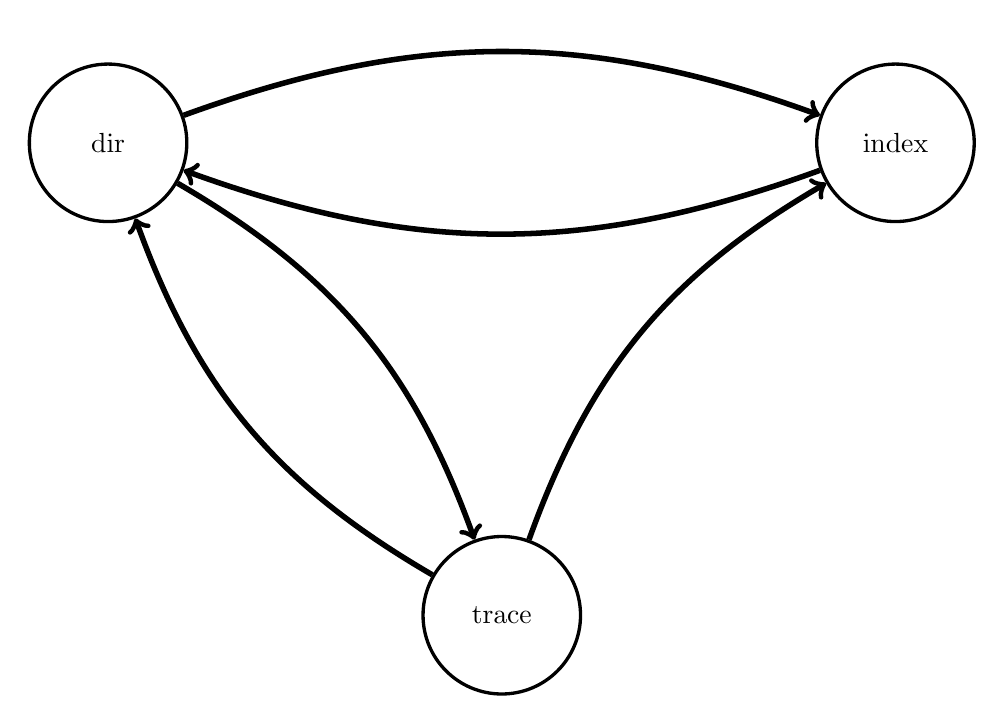
\begin{tikzpicture}[
    state/.style={draw = black, circle, minimum width = 2cm, very thick},
    arrow/.style={black, ->, line width = 2pt}
  ]
\begin{scope}[on grid]
\node[state] (dir)   {dir};
\node[state] (trace) [below right=6cm and 5cm of dir] {trace};
\node[state] (index) [right=10cm of dir] {index};
\end{scope}

\path (dir)   edge [arrow, bend right = -20] node [midway, above] {\gufidirindex}   (index);
\path (index) edge [arrow, bend left  =  20] node [midway, above] {\gufiindexdir}   (dir);

\path (dir)   edge [arrow, bend right = -20] node [midway, below] {\gufidirtrace}   (trace);
\path (trace) edge [arrow, bend left  =  20] node [midway, below] {\gufitracedir}   (dir);

\path (trace) edge [arrow, bend right = -20] node [midway, below] {\gufitraceindex} (index);
\end{tikzpicture}
\caption{Tools for Transforming Between Source Trees, Traces, and Indexes}
\end{figure}

\subsubsection{\gufitracedir}
\paragraph{Flags}
\begin{table} [H]
  \centering
  \begin{tabular}{l|l}
    Flag & Functionality \\
    \hline
    -h & help manual \\
    \hline
    -H & Show assigned input values \\
    \hline
    -n \textless num\_threads\textgreater & define number of threads to use \\
    \hline
    -d \textless delim\textgreater & delimiter (one char)  [use 'x' for 0x1E] \\
    \hline
    -x & pull xattrs from source file-sys into GUFI \\
    \hline
  \end{tabular}
  \caption{\gufitracedir Flags and Arguments}
\end{table}

\paragraph{Usage} ~\\\\
\gufitracedir \texttt{[options] trace\_file... output\_dir}

\subsubsection{\gufiindexdir}
\paragraph{Flags}
\begin{table} [H]
  \centering
  \begin{tabular}{l|l}
    Flag & Functionality \\
    \hline
    -h & help manual \\
    \hline
    -H & Show assigned input values \\
    \hline
    -n \textless num\_threads\textgreater & define number of threads to use \\
    \hline
    -x & pull xattrs from source file-sys into GUFI \\
    \hline
  \end{tabular}
  \caption{\gufiindexdir Flags and Arguments}
\end{table}

\paragraph{Usage} ~\\\\
\gufiindexdir \texttt{[options] input\_dir output\_dir}


\include{sections/implementation}

\end{document}
